In this Section, the results of the analysis of the galaxy properties in TNG is presented, along with comparisons to observational data.

\subsection{Stellar-to-halo-mass relation}

The first relation that is studied is the stellar-to-halo-mass relation. It is one of the most fundamental relations that a hydrodynamical cosmological simulation should reproduce, as it ensures that we have the right distribution of halos and galaxies in our mock universe. This relation depends sensitively on the stellar mass content in the galaxy sample, and as such on the stellar mass definition used. The results for the fractional difference in stellar mass measurements as a function of halo mass for different definitions of galaxy radius are presented in Figure \ref{HM_fSM}. The most obvious result is the significant difference between $M_\ast^{SUBF}$ and $M_\ast^{2rhm}$, with the latter being at least 20 \% smaller for all stellar masses. $M_\ast^{15r200}$ and $M_\ast^{30kpc}$ are essentially indistinguishable from the SUBFIND values at halo masses below $10^{12} M_{\odot}$. For more massive galaxies there is an increasingly large difference between the two as well as compared to SUBFIND. At the higher mass end ($M_{halo} > 10^{13} M_{\odot}$), $M_\ast^{15r200}$ is about 10-15 \% smaller than SUBFIND, $M_\ast^{30kpc}$ is 12-40 \% smaller while $M_\ast^{2rhm}$ is approximately 30 \% smaller.


\begin{figure}
    \centering
    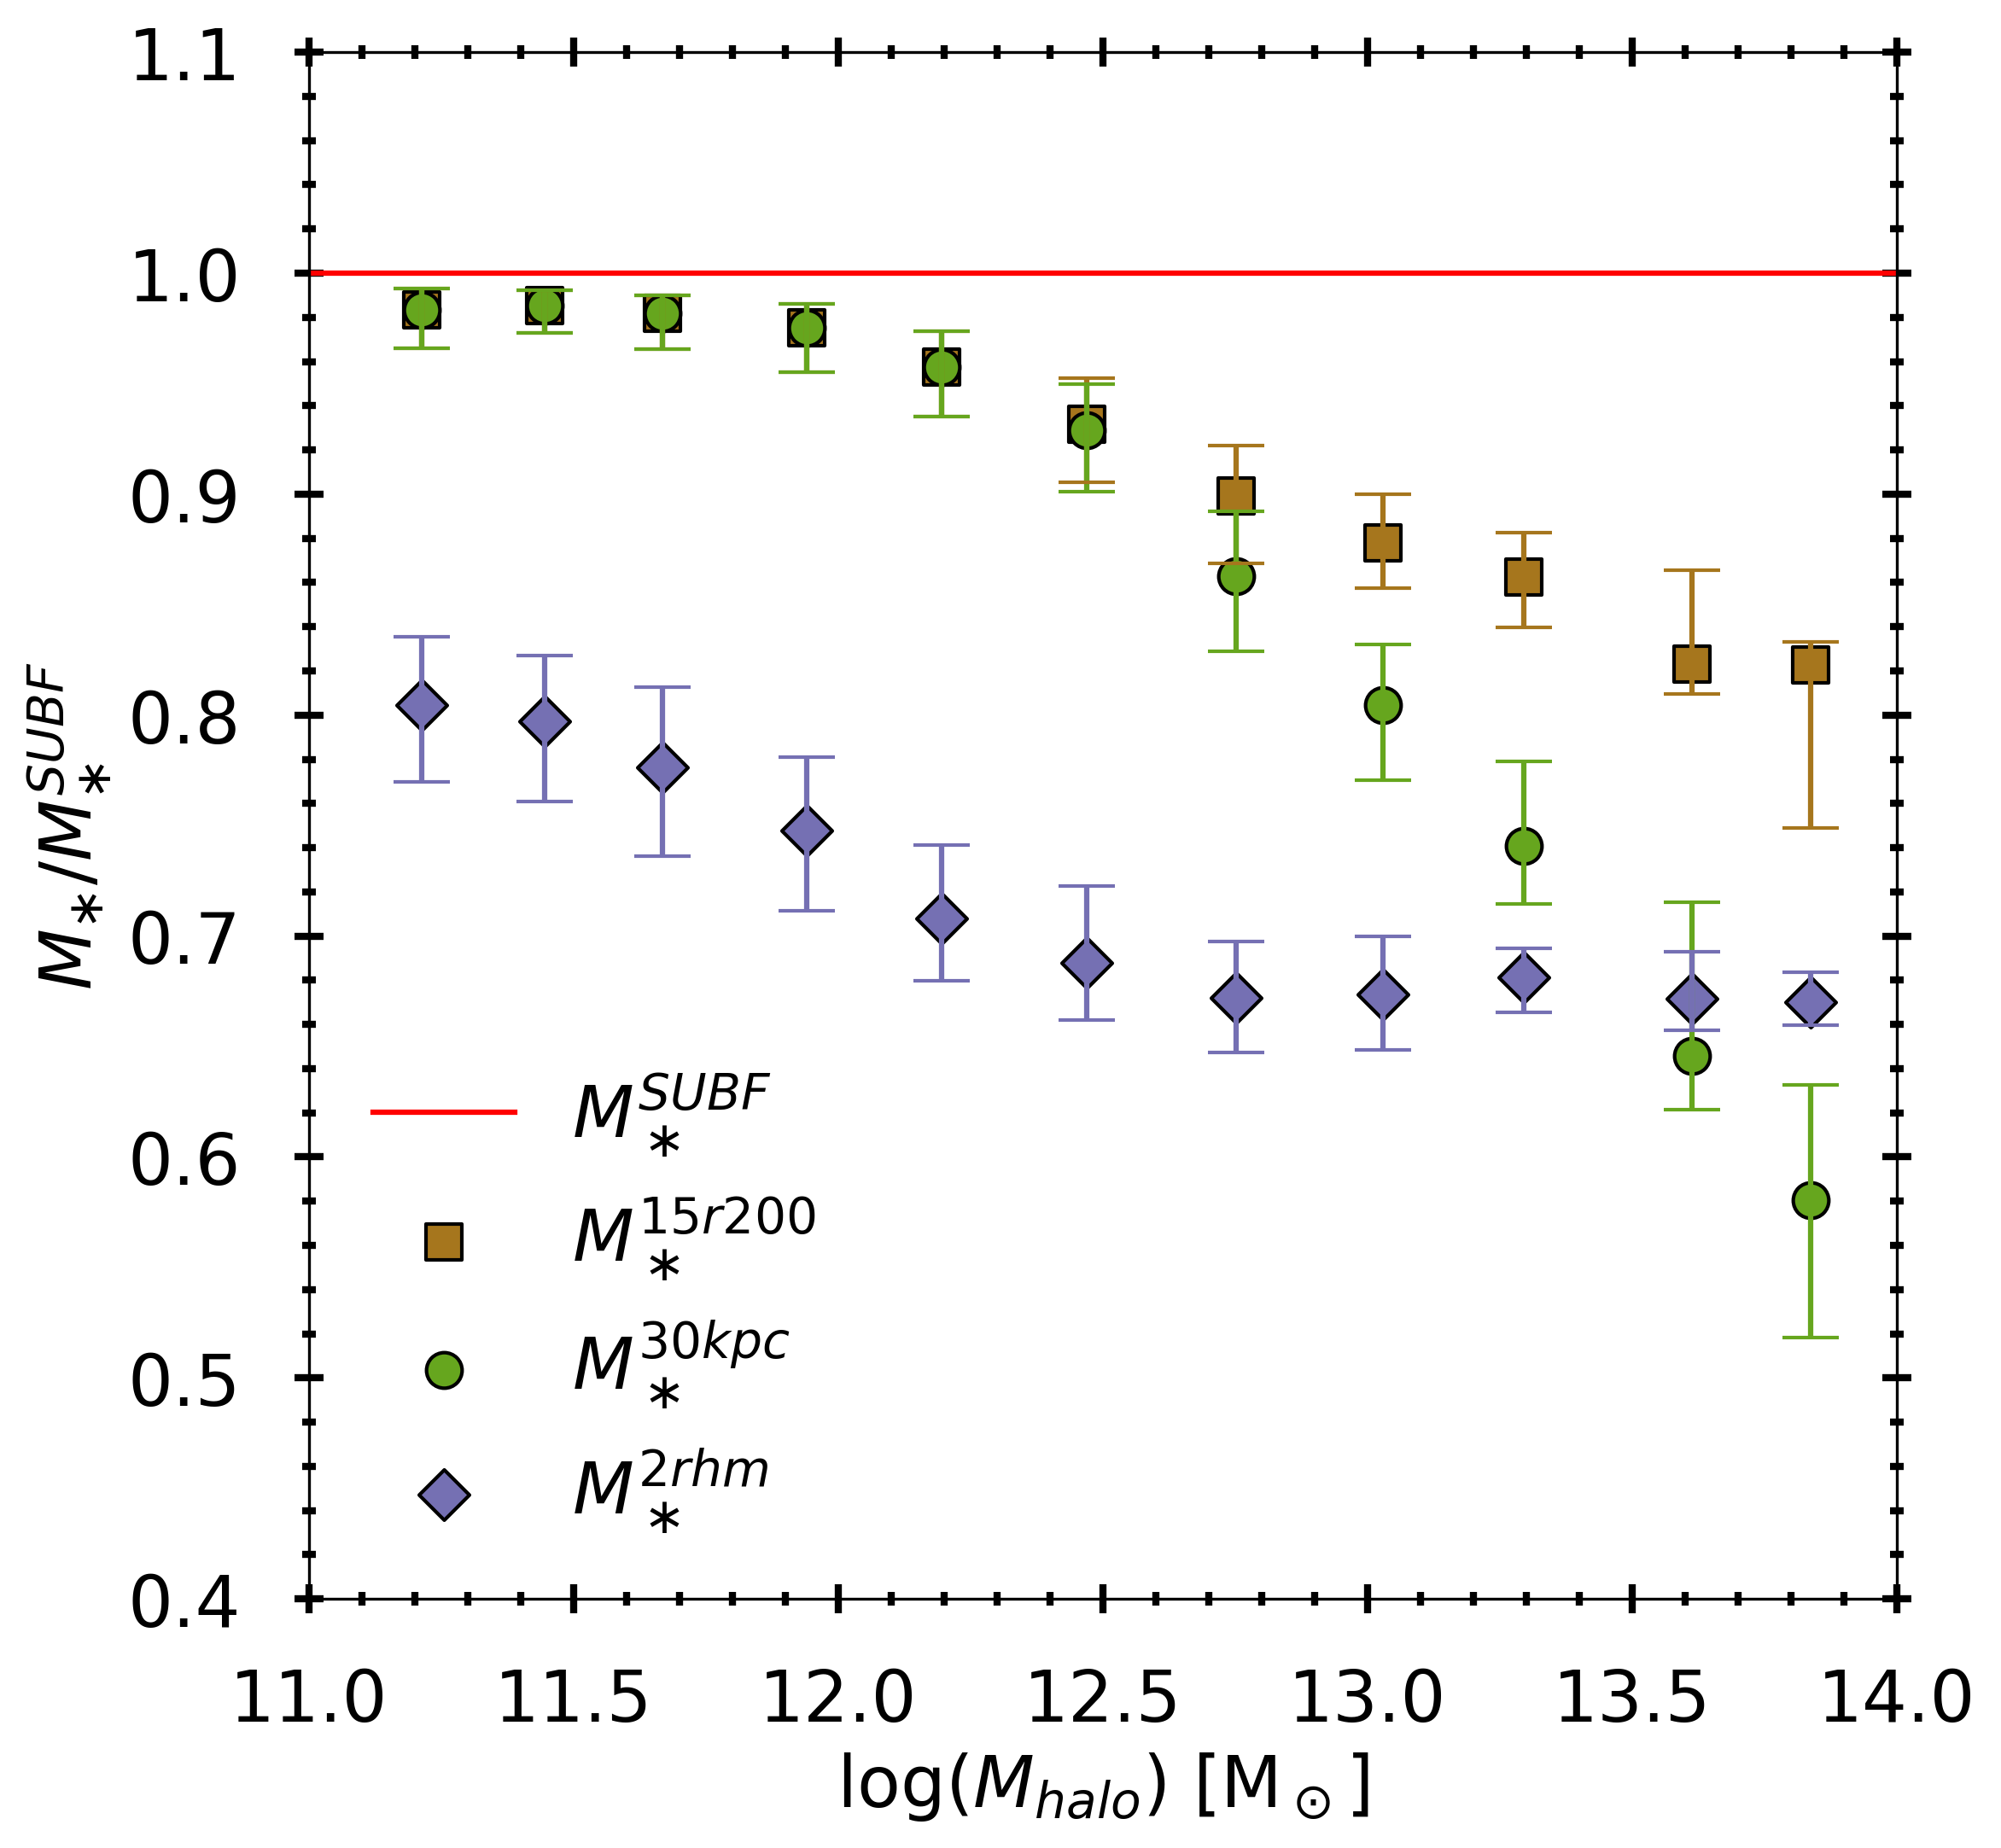
\includegraphics[width=0.9\textwidth]{images/HM_fSM.png}
    \caption{The fractional difference between the stellar mass of the galaxy using different definitions of galaxy size and the total mass of all stellar particles bound to the subhalo as identified by SUBFIND as a function of halo mass. Median values with 25-75 percentile error bars are given for the stellar mass within 15 \% of the virial radius ($M_\ast^{15r200}$, orange squares), within 30$\,$ kpc ($M_\ast^{30kpc}$, green circles) and within twice the SUBFIND half mass radius ($M_\ast^{2rhm}$, purple diamonds)}
    \label{HM_fSM}
\end{figure}


In Figure \ref{shmr} the SHM relation is shown for the different definitions of stellar mass in TNG ($M_\ast^{15r200}$ is left out to make the figure more readable) along with the best fits from \textcite{Behroozi2019}, \textcite{Zanisi2019} and \textcite{Kravtsov2018}. The two former use abundance matching while the latter uses empirically found stellar and halo masses for galaxy clusters. $M_\ast^{2rhm}$ deviates the most from the slope of the observational data, neither matching the low nor high mass end. $M_\ast^{30kpc}$ and $M^{SUBF}_\ast$ match the observations well at low halo masses, but the become too steep at halo masses of about $10^{13} M_\odot$. The 30 kpc aperture produces a slope that is more similar to observations than using all the bound particles. All the different definitions overestimate the stellar mass compared to \textcite{Behroozi2019} and \textcite{Zanisi2019} observations for the most massive halos with $M_{halo} > 10^{13.5} M_\odot$. \textcite{Kravtsov2018} values are similar to the $M^{SUBF}_\ast$ values at these high masses, but the TNG slope is still steeper. 

\begin{figure}
    \centering
    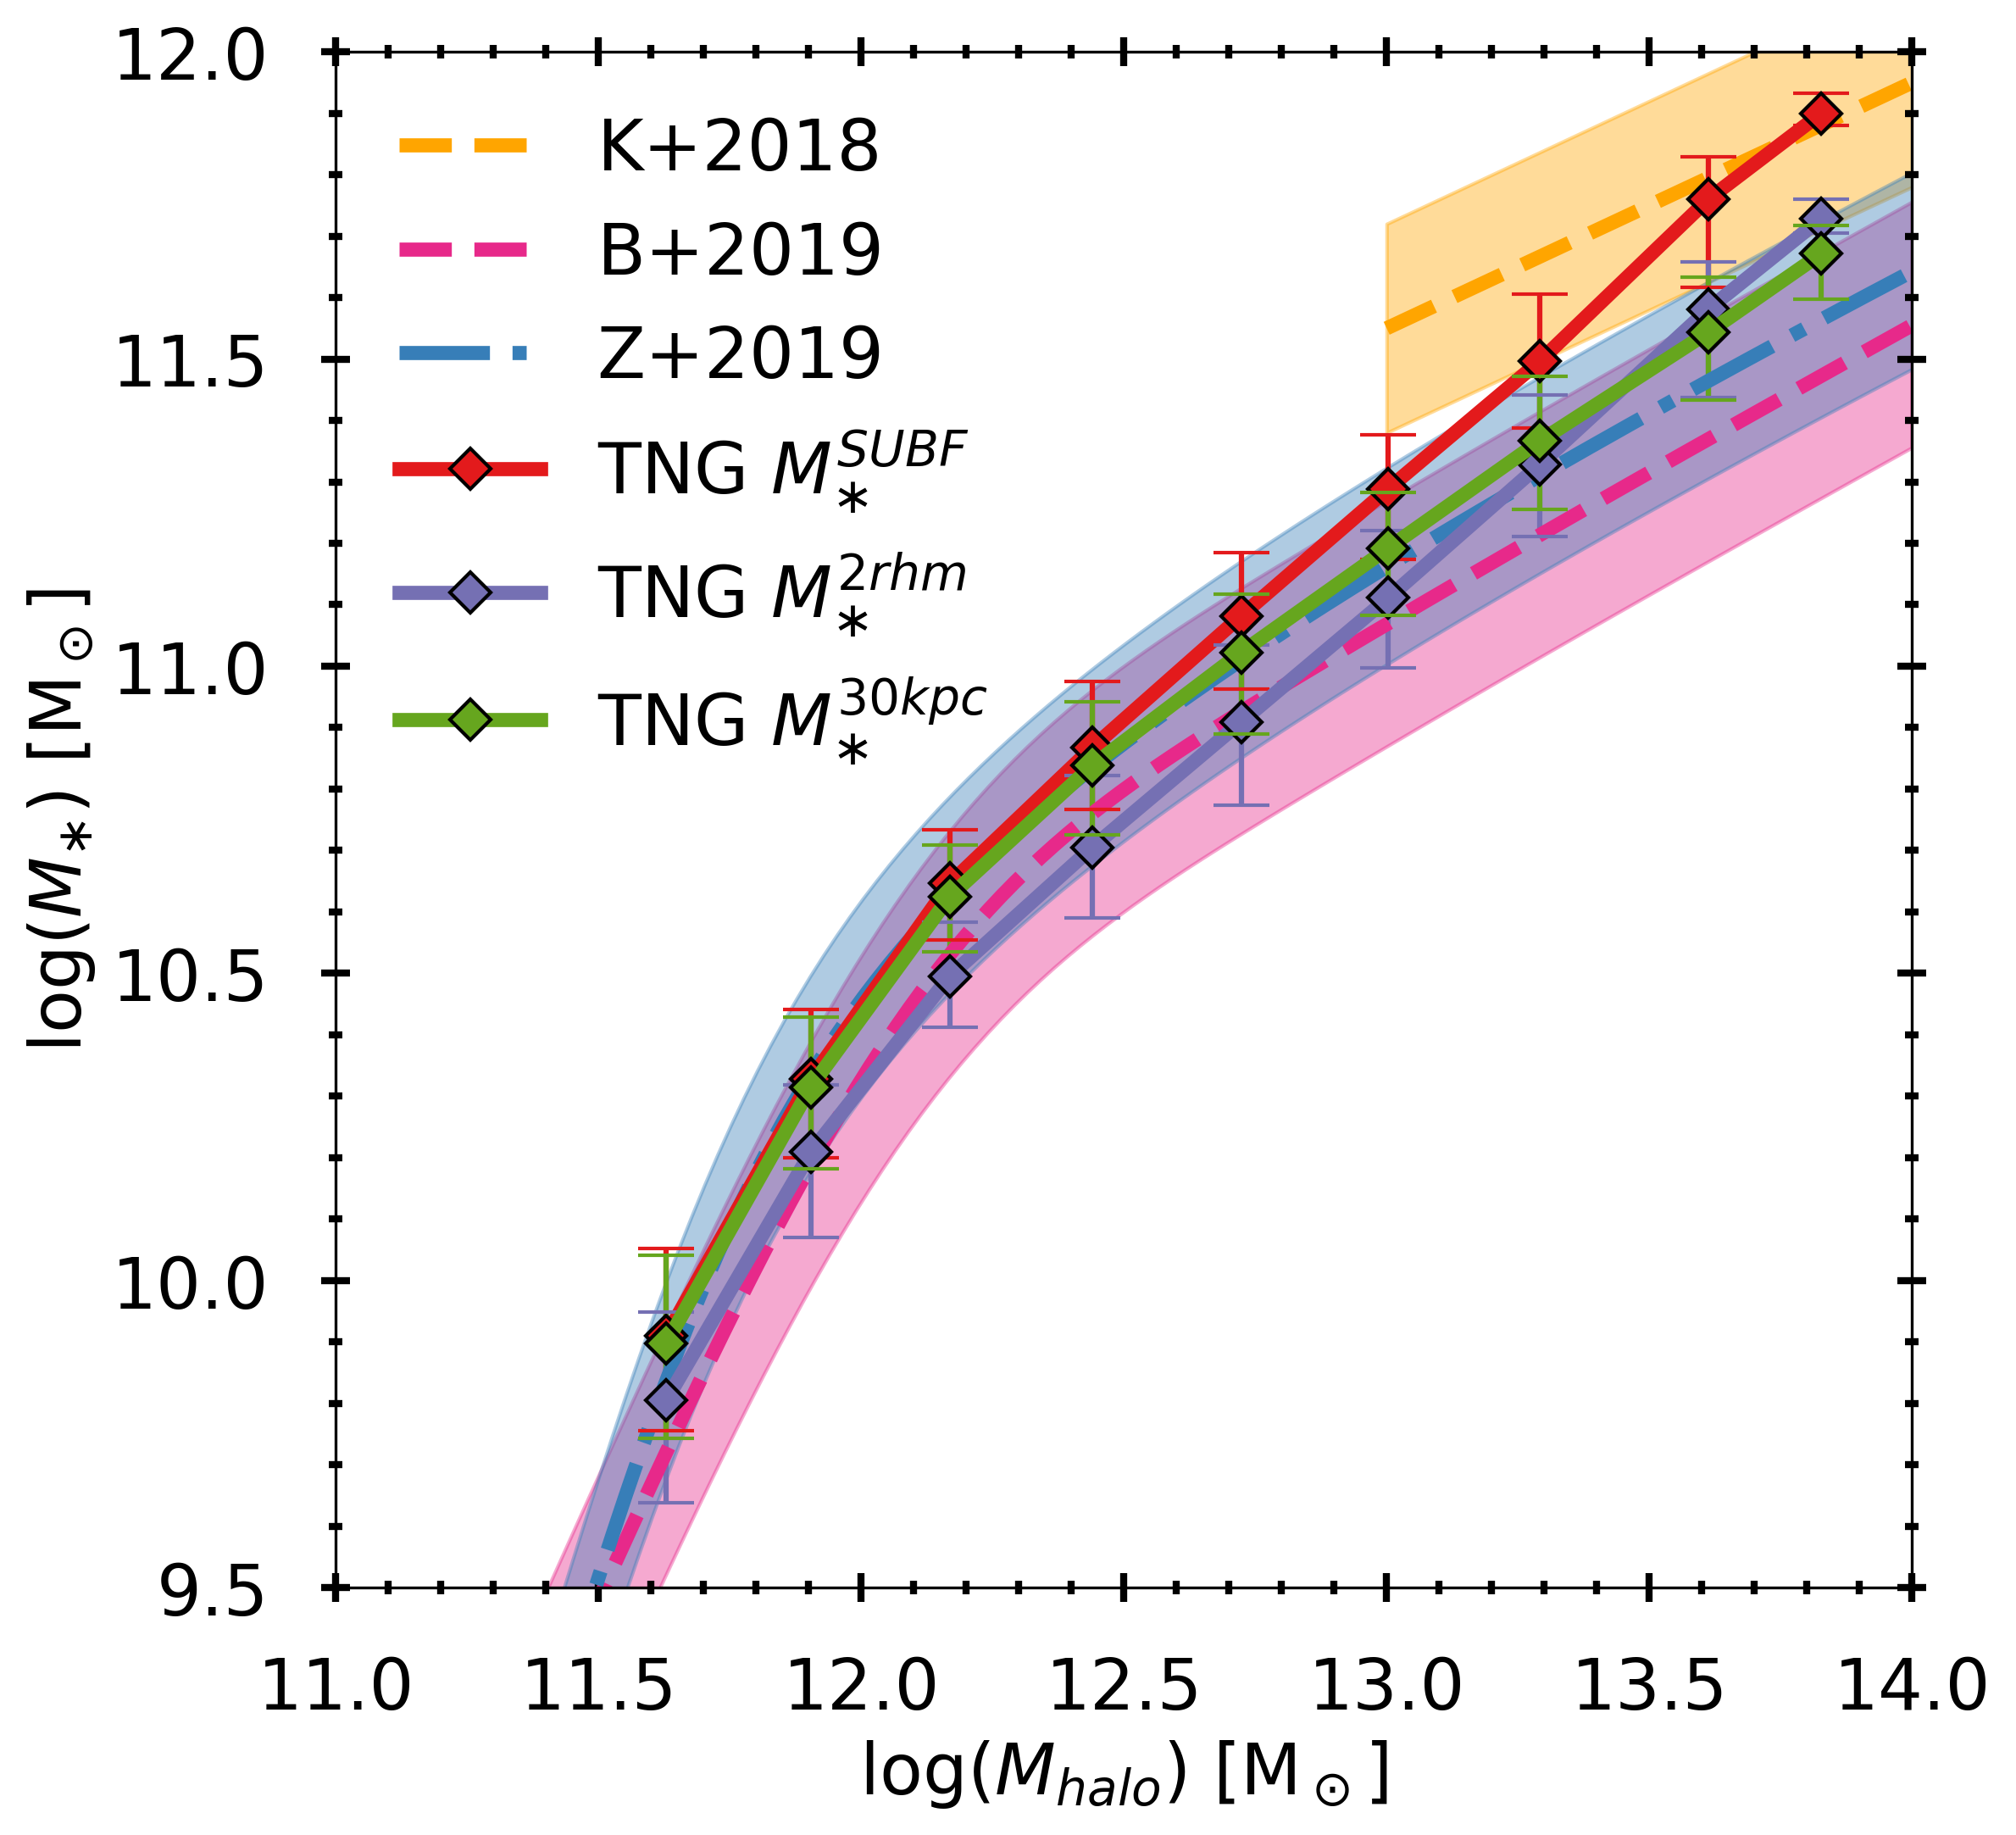
\includegraphics[width=0.9\textwidth]{images/shmr.png}
    \caption{The SHM relation of TNG for three different mass definitions, the stellar mass in the entire subhalo ($M_\ast^{SUBF}$, red), within 30$\,$ kpc ($M_\ast^{30kpc}$, green) and within twice the SUBFIND half mass radius ($M_\ast^{2rhm}$, purple). The diamond markers indicate median points and include error bars showing the 25-75 percentile. The best fit from abundance matching from \textcite{Behroozi2019} (pink dashed line), \textcite{Zanisi2019} (blue long-dashed line) and \textcite{Kravtsov2018} (orange dashed line) are also shown.}
    \label{shmr}
\end{figure}


\subsection{Characteristic size and velocities}
After looking at the SHM relation, the next fundamental galaxy relations that were studied are those relating to the structure and kinematics of the galaxies. Firstly, the stellar mass-size relation gives us an idea about the distribution of the stellar mass within the subhalo. The relation is studied for the entire galaxy population as well as for early and late type galaxies. Next, the velocity measurements of early and late type galaxies as functions of stellar mass give insight into the total mass distribution in the subhalos. Specifically the Tully-Fisher and Faber-Jackson relation are studied and the TNG data are compared against observations.

\subsubsection{Mass-size}
The half-mass radius will of course be affected by the definition of stellar mass, as it is defined as the radius within which half the stellar mass of the galaxy is found. This can be seen in Figure \ref{SM_R_TNG}, in which the stellar half-mass radius $r_{hm}$ and the projected half-mass radius $R_{hm}$ are plotted for different galaxy size definitions as a function of the subhalo stellar mass $M^{SUBF}_\ast$. There is a large scatter in this function, and the resulting trends lie within the 25-75 percentile of each other. However, it is still clear that there is a difference in the slope of the relation for the $M_\ast > 10^{11} M_{\odot}$ regime. $r^{SUBF}_{hm}$ is larger than $r^{15r200}_{hm}$ by up to 0.1 dex and larger than $r^{30kpc}_{hm}$ by up to 0.2 dex for the most massive galaxies. %gives these numbers (differences) in %

It is also interesting to compare the two methods of calculating projected 2D half-mass radii. For the SUBFIND catalog the relation $R_{e} \approx 3/4 \times r_{e}$ is used to approximate the projected radius (see Section \ref{charsize}). When using the particles, one can project the galaxies in three orthogonal directions and calculate the average 2D half-mass radius. The results show that multiplying by a factor of $3/4$ is an excellent approximation to the projected stellar half-mass radius (see dashed line on Figure \ref{SM_R_TNG}).

In Figure \ref{SM_R}, the TNG projected half mass radii as a function of stellar mass (using the 30 kpc aperture as well as all bound particles) for the entire galaxy sample is compared against the data from the SAMI survey. The TNG simulation produces galaxies with half-mass radii that are slightly larger than the SAMI effective radii at lower stellar masses. At high stellar masses the SUBFIND values are higher than those of the fixed aperture of 30 kpc and is a better fit for the Sèrsic-fit effective radius observational data, while $R_{hm}^{30kpc}$ is a better fit for the $R_{e, mge}$ values. TNG galaxies also show a flat or negative slope in the mass range $10^{9.5} M_{\odot} - 10^{10.5} M_{_\odot}$, while the SAMI data has a positive slope such that more massive galaxies have increasingly larger radii across the mass spectrum.


The stellar mass-size relation for early and late type galaxies is shown in Figure \ref{SM_R_earlies} and Figure \ref{SM_R_lates} respectively. %tell here what each panel mean
The half-mass radii for late type galaxies are larger than for early types with similar mass, as expected. The relation is sensitively dependent on the criteria used in morphology classifications. In Figure \ref{SM_R_earlies} the SAMI early type galaxies show different behaviours for different morphology classifications in the low mass range. Including the S0 galaxies smoothes out the curve. The galaxy sample is very small %how small?
in this range though, so this might just be statistical deviations in the mean values. For TNG, the relation does not change significantly based on whether or not the $\kappa_{rot}$ criteria is used. 
For late type galaxies however (Figure \ref{SM_R_lates}) there is a big difference in TNG data. The galaxy sizes of the least massive galaxies increase when the $\kappa_{rot}$ criteria is added. For SAMI data the opposite happens when ``early spirals'' are included in the late type category, the size goes down. This is expected, as more spherical galaxies are smaller than disk-shaped galaxies. Thus, the SAMI ``early + late spirals'' and the TNG $\log(sSFR) > -1.44$ sample are the most similar in the late type size-mass relation. For the early type size-mass relation, the TNG morphology criteria does not matter, but the ``elliptical + S0'' SAMI sample matches better the TNG data.


\begin{figure}
    \centering
    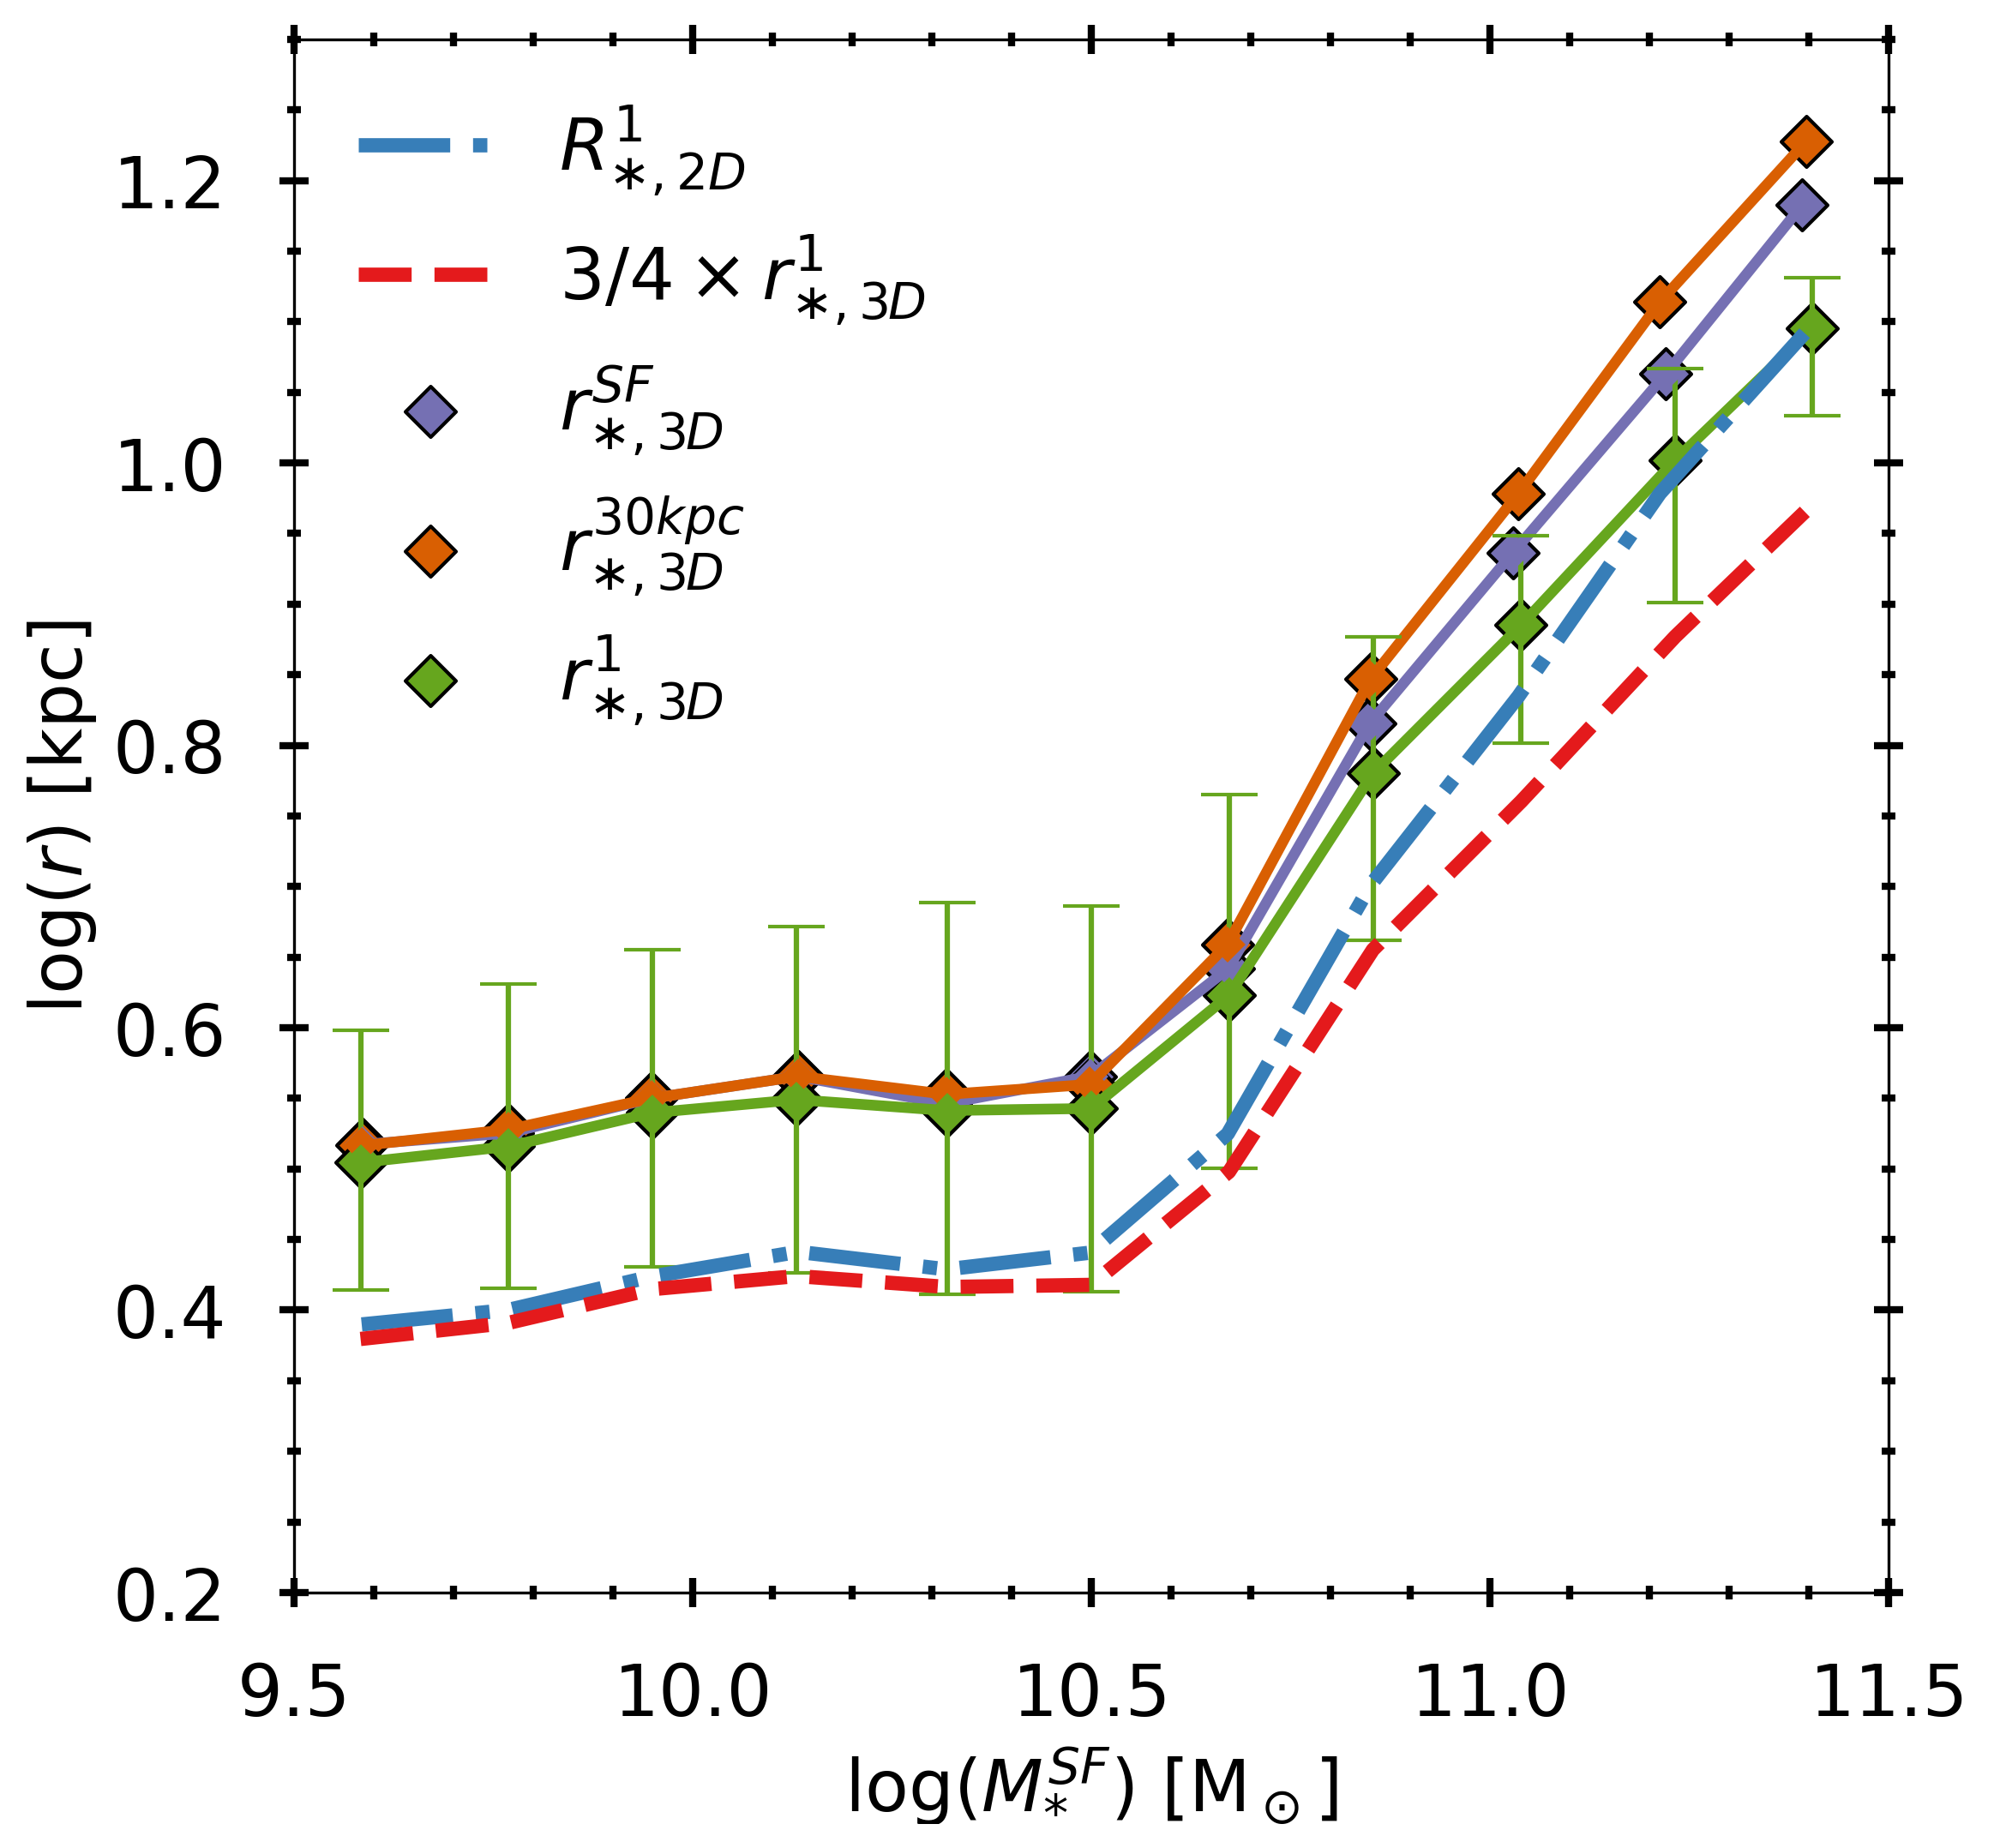
\includegraphics[width=0.9\textwidth]{images/SM_R_tng.png}
    \caption{The size-mass relation for three different galaxy size definitions in TNG, the half-mass radius for the stellar mass in the entire subhalo ($r_{hm}^{SUBF}$, red), the stellar mass within 15 \% of the virial radius (($r_{hm}^{15r200}$, red), orange squares), within 30$\,$ kpc (($r_{hm}^{30kpc}$, red), green circles). The half-mass radii are all plotted as functions of the total SUBFIND stellar mass $M^{SUBF}_\ast$. The 2D projected radius $R_{hm}^{15r200}$ and the estimated 2D projected radius $3/4 \times r_{hm}^{15r200}$ are also shown as purple and green dashed lines respectively. The 25-75 percentile error bars are shown for $r^{15r200}_{hm}$ only, as the scatter is similar for all definitions.}
    \label{SM_R_TNG}
\end{figure}


\begin{figure}
    \centering
    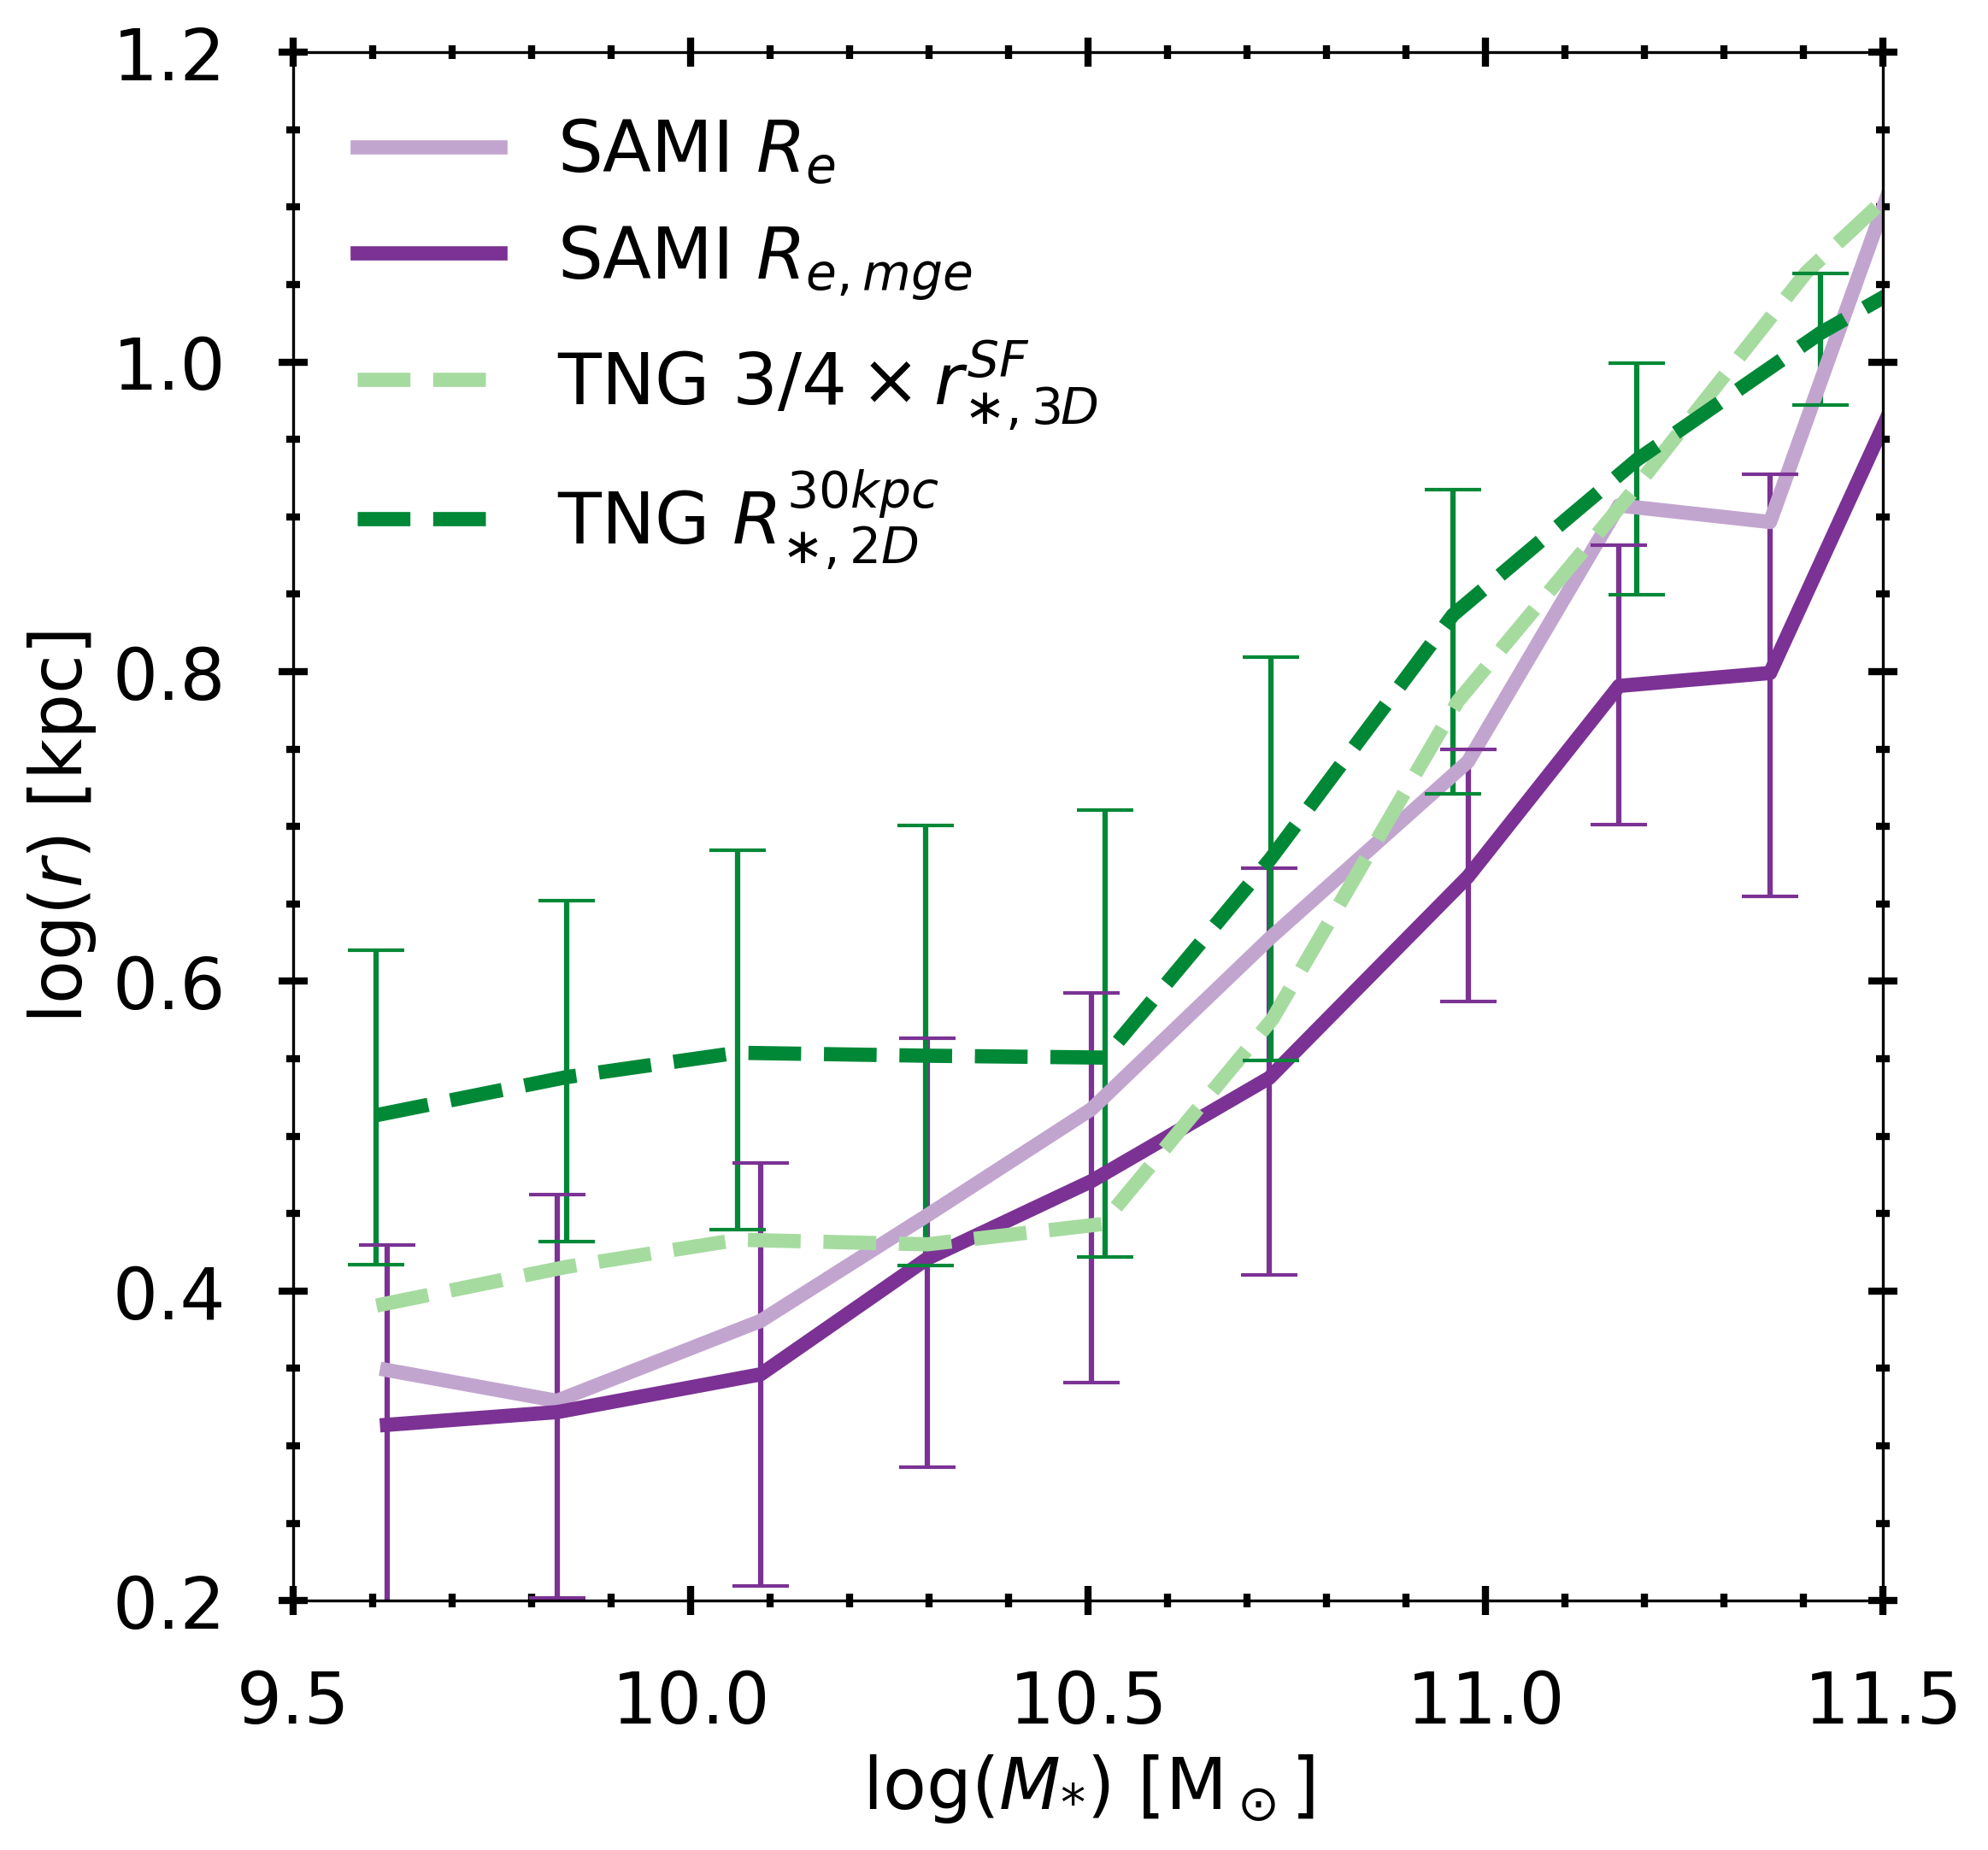
\includegraphics[width=0.9\textwidth]{images/SM_R.png}
    \caption{The size-mass relation of the whole galaxy sample in both TNG and SAMI, given by median values with corresponding 25-75 percentile error bars. TNG values are shown in green dashed lines, while SAMI values are the purple solid lines.}
    \label{SM_R}
\end{figure}


\begin{figure}
    \centering
    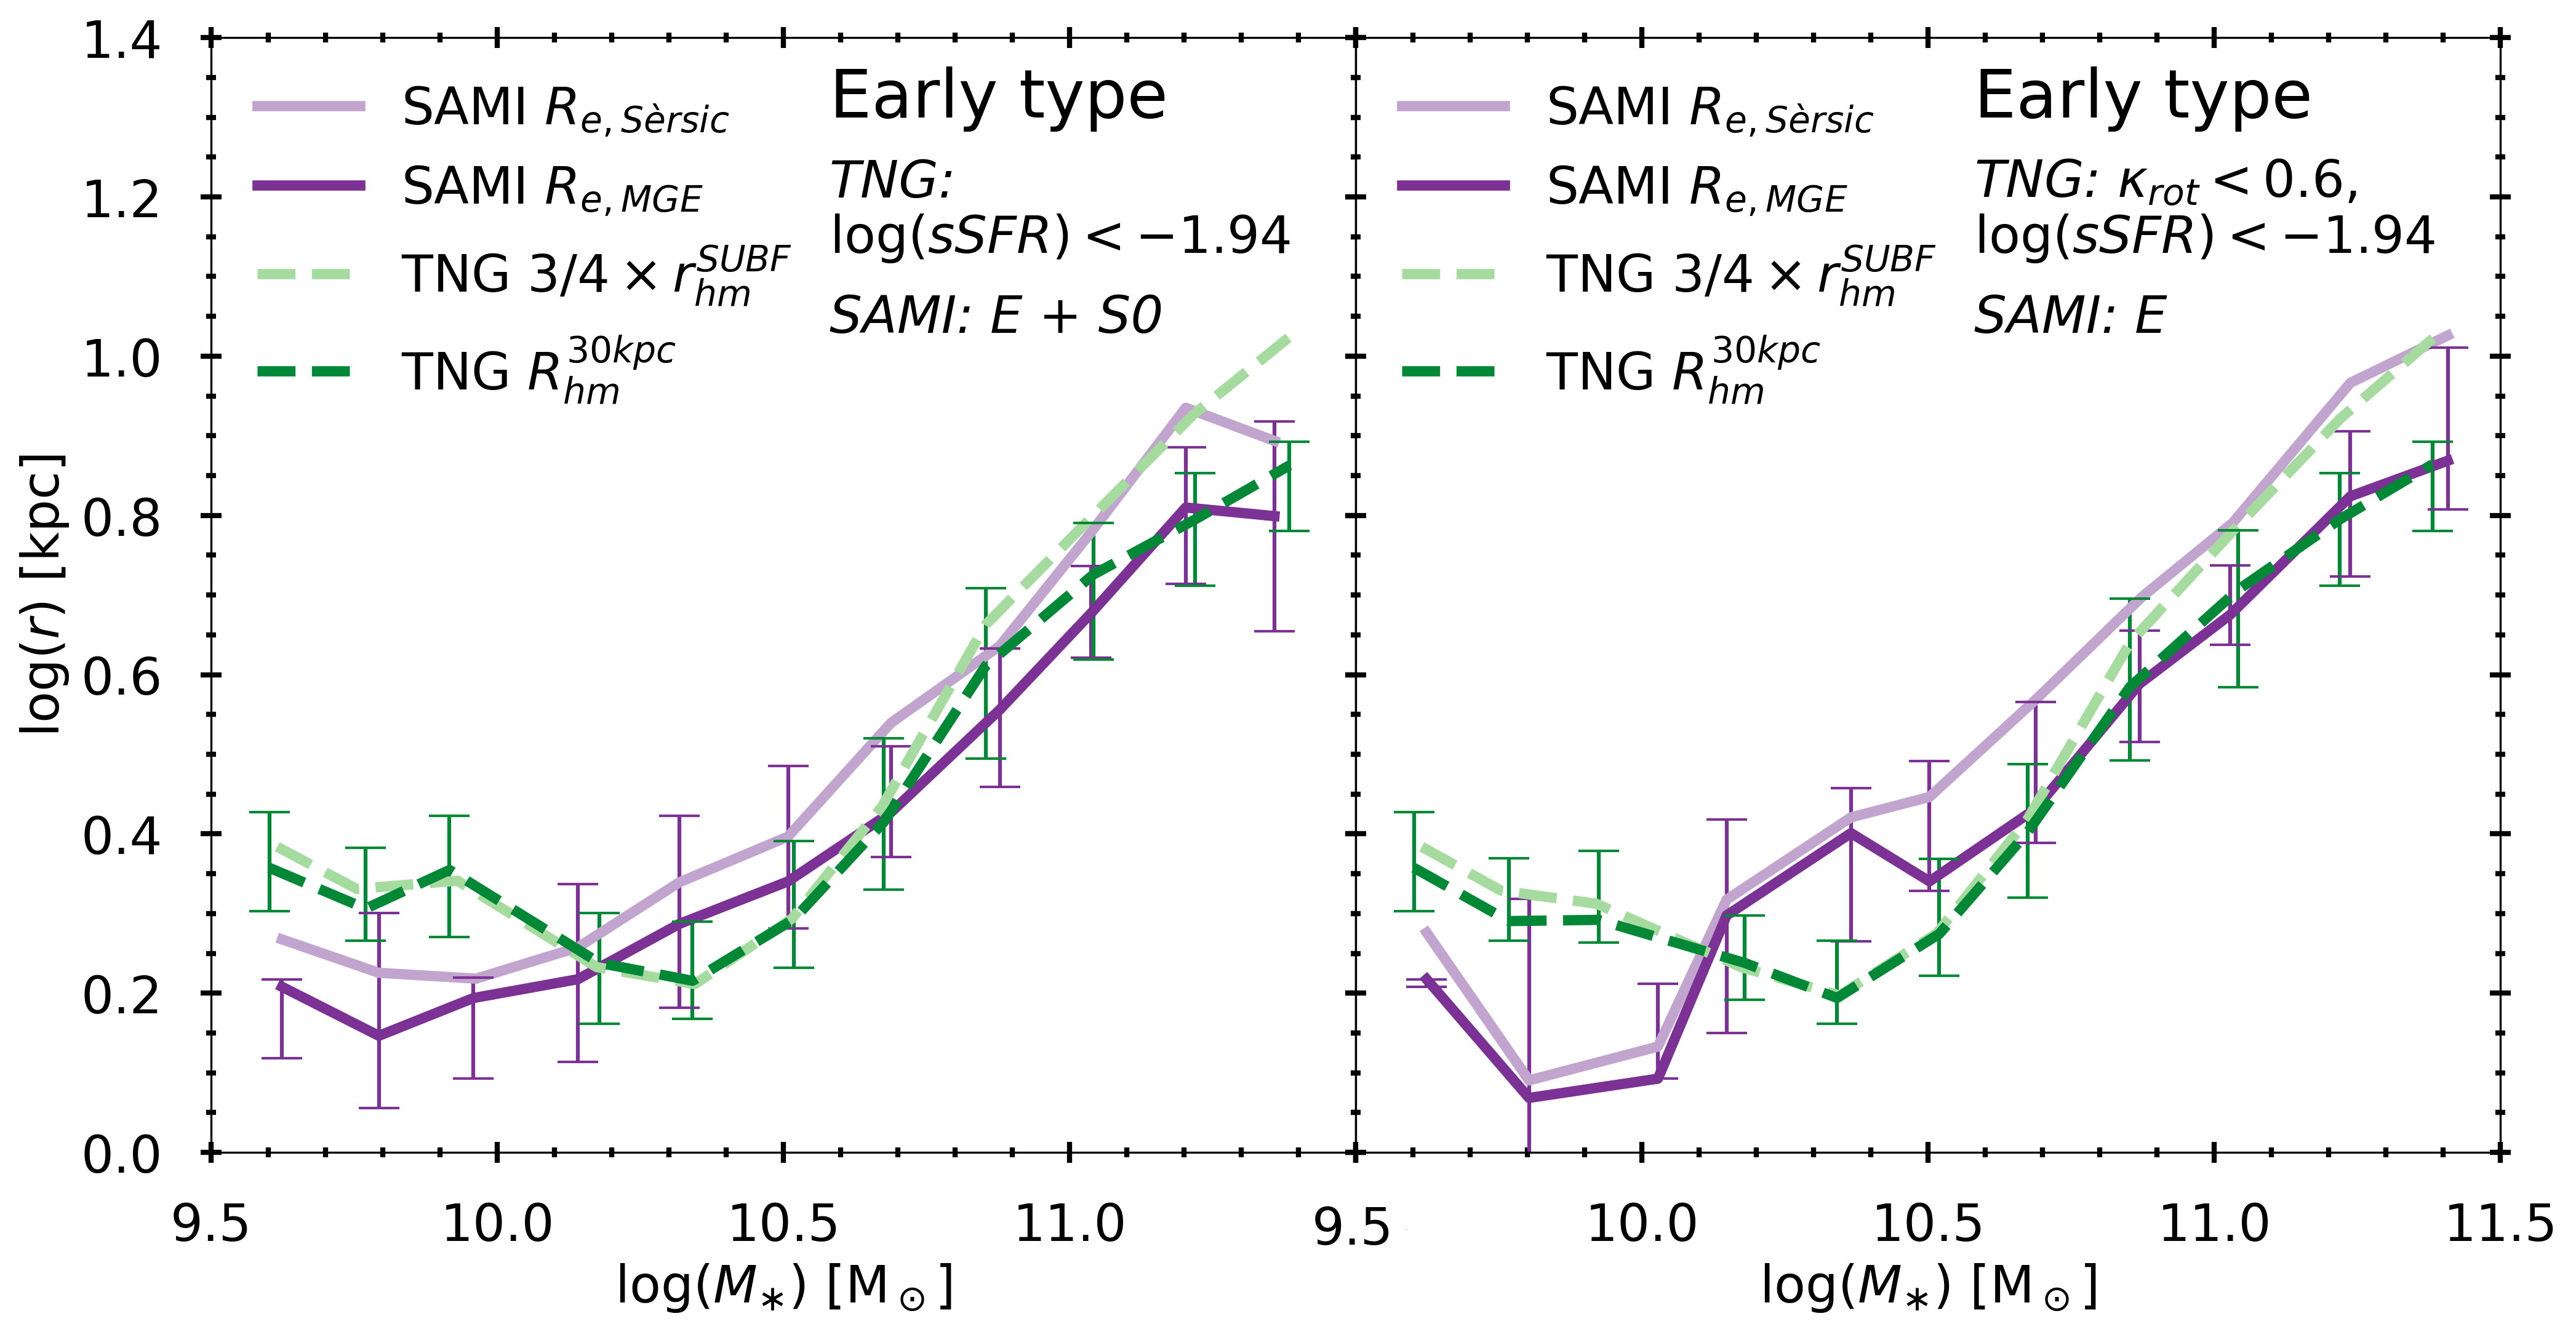
\includegraphics[width=\textwidth]{images/SM_R_earlies.png}
    \caption{The size-mass relation of early type galaxies in both TNG and SAMI, given by median values with corresponding 25-75 percentile error bars. TNG values are shown in green dashed lines, while SAMI values are the purple solid lines. The two panels show the effect of the morphology selection criteria. Left: TNG galaxies with $\log(sSFR) < -1.94$ and SAMI elliptical and S0 galaxies. Right: TNG galaxies with $\log(sSFR) < -1.94$ as well as $\kappa_{rot} < 0.6$ and SAMI elliptical galaxies.}
    \label{SM_R_earlies}
\end{figure}

\begin{figure}
    \centering
    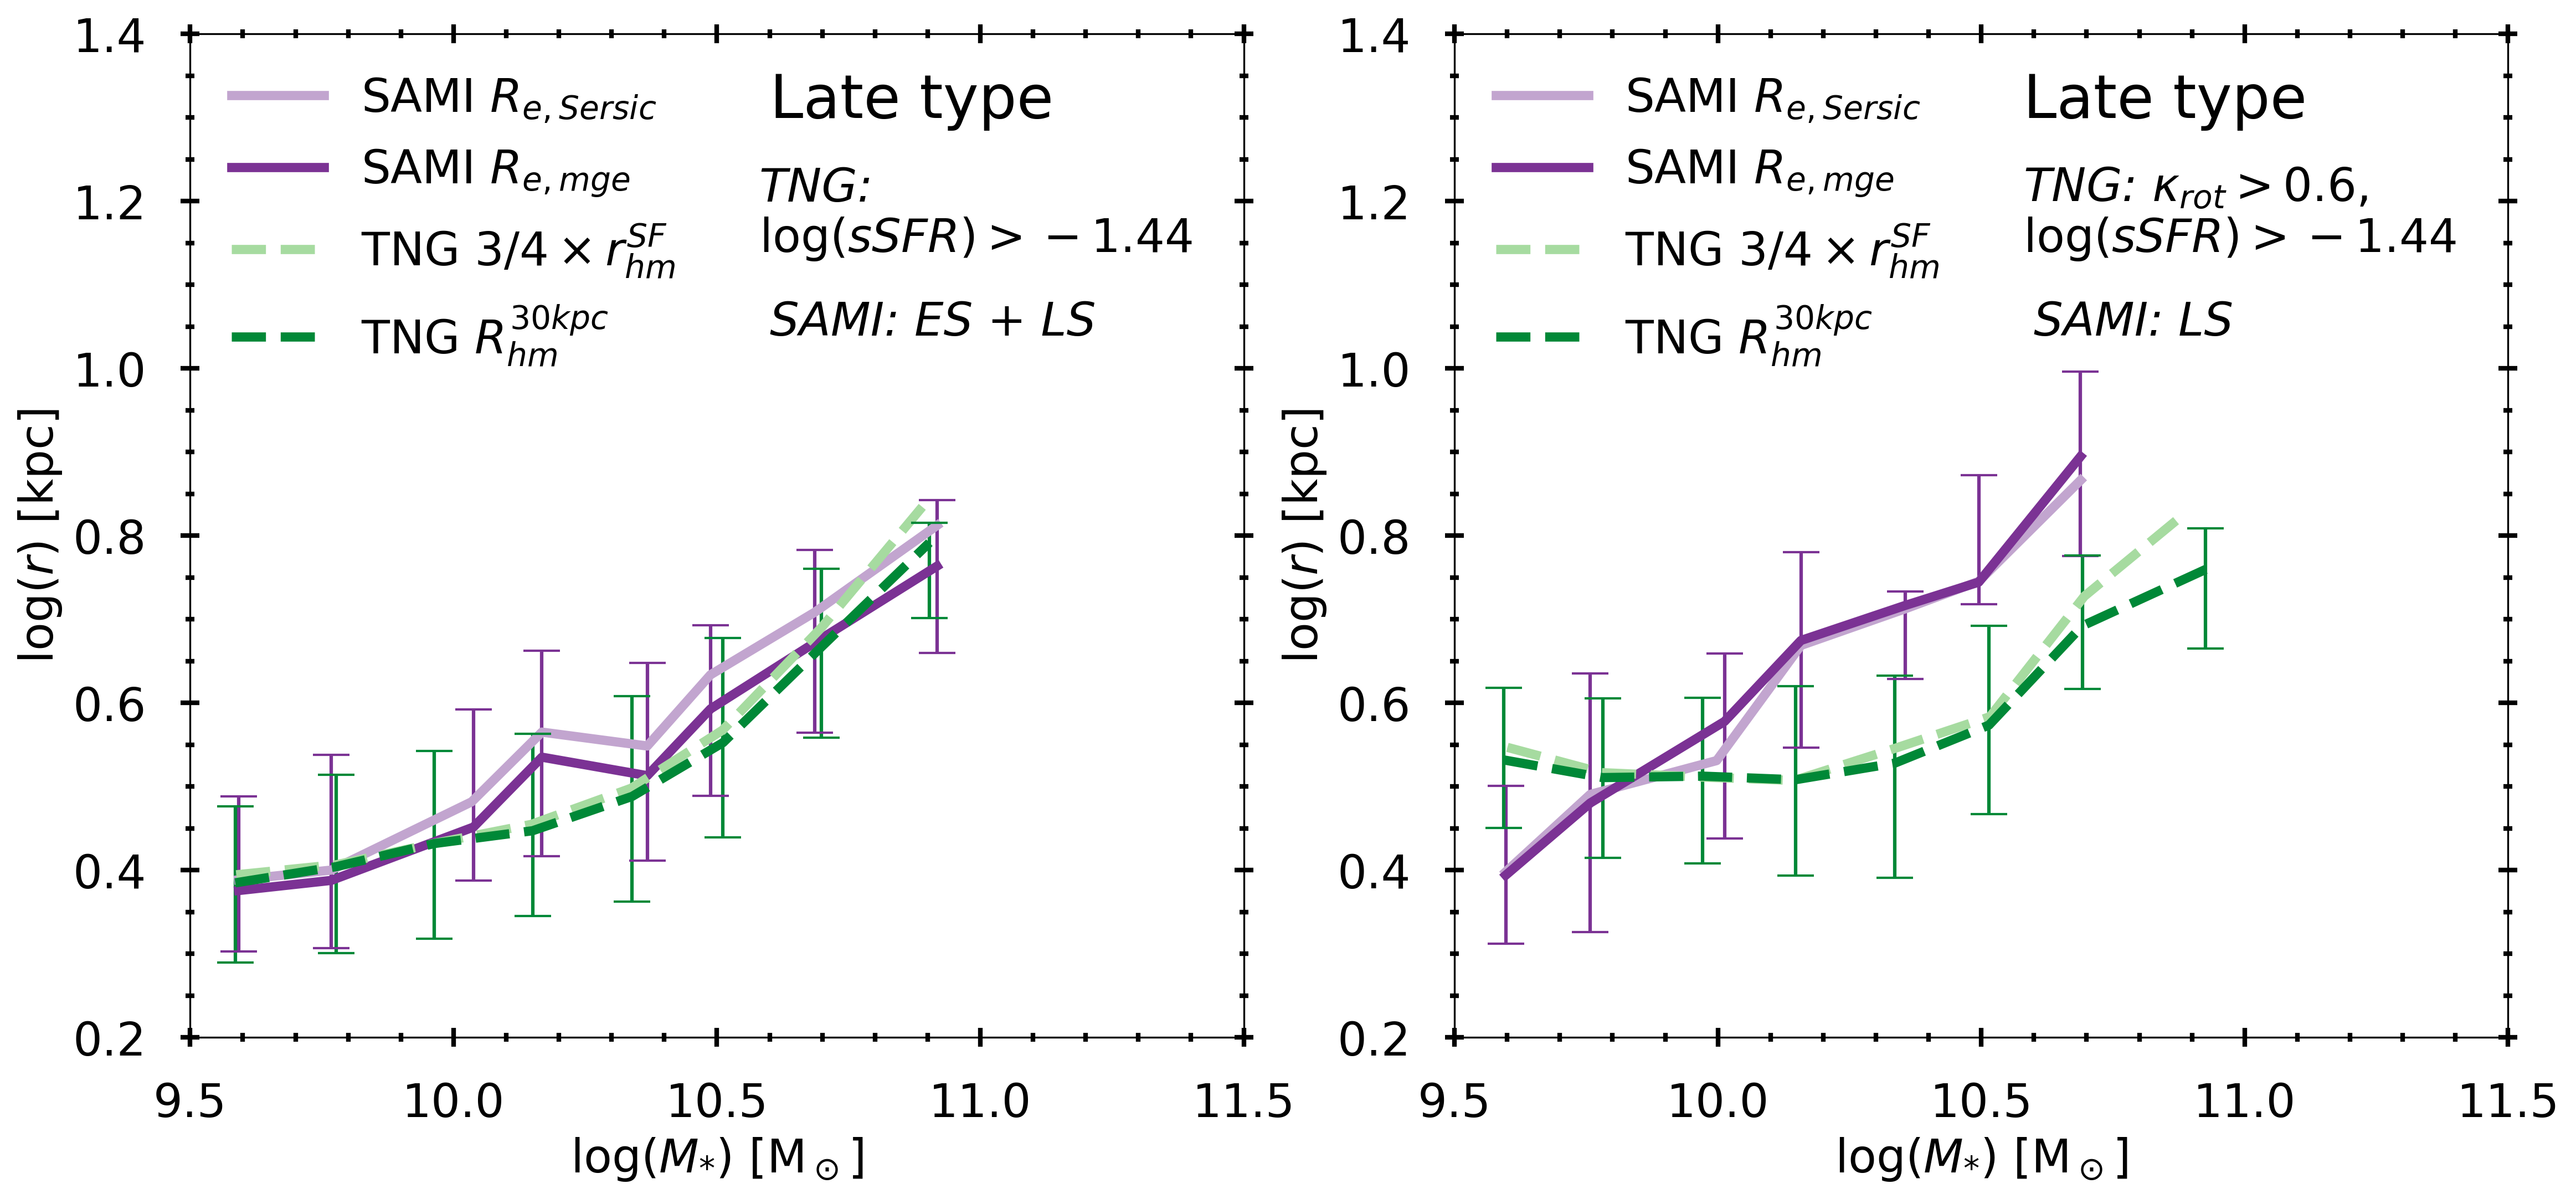
\includegraphics[width=\textwidth]{images/SM_R_lates.png}
    \caption{The size-mass relation of late type galaxies in both TNG and SAMI, given by median values with corresponding 25-75 percentile error bars. TNG values are shown in green dashed lines, while SAMI values are the purple solid lines. The two panels show the effect of the morphology selection criteria. Left: TNG galaxies with $\log(sSFR) > -1.44$ and SAMI early and late spiral galaxies. Right: TNG galaxies with $\log(sSFR) > -1.44$ as well as $\kappa_{rot} > 0.6$ and SAMI late spiral galaxies.}
    \label{SM_R_lates}
\end{figure}

\subsubsection{Mass - rotational velocity}
As the SUBFIND catalog value for rotational velocity is the maximum of the spherically averaged rotation curve, it was interesting to see if the rotational velocities are significantly smaller at specific radii where observational measurements are made. To test this, the rotational velocity was calculated at a radius of $2.2 \times r_{hm}$. There was no difference in the produced data. At that distance the velocity curve is well into the flat regime caused by the dark matter halo, and so this shows that the maximum rotational velocity is not much different from the flat part.

In Figure \ref{TFR} the Tully-Fisher relation is shown for TNG, along with the best-fit from the SAMI data by \textcite{Bloom2017} and CALIFA data by \textcite{Bekerait2016} who calculated their velocities at $2.2 \times R_e$ and at the radius within 83\% of the light is contained respectively. Both measurements are within the flattened part of the velocity curve, and so they should be comparable. The TNG data is calculated using a galaxy size of 30 kpc and rotational velocities measured at $2.2 \times r_{hm}^{30kpc}$. The SAMI data has a steeper slope than the TNG data, being 0.31 and 0.25 respectively. The CALIFA study has a slope of 0.27 $\pm 0.13$, but a lower zero point, and so the TNG results lie between the CALIFA and SAMI fits for $M_\ast > 10^{10}M_{\odot}$. 


\begin{figure}
    \centering
    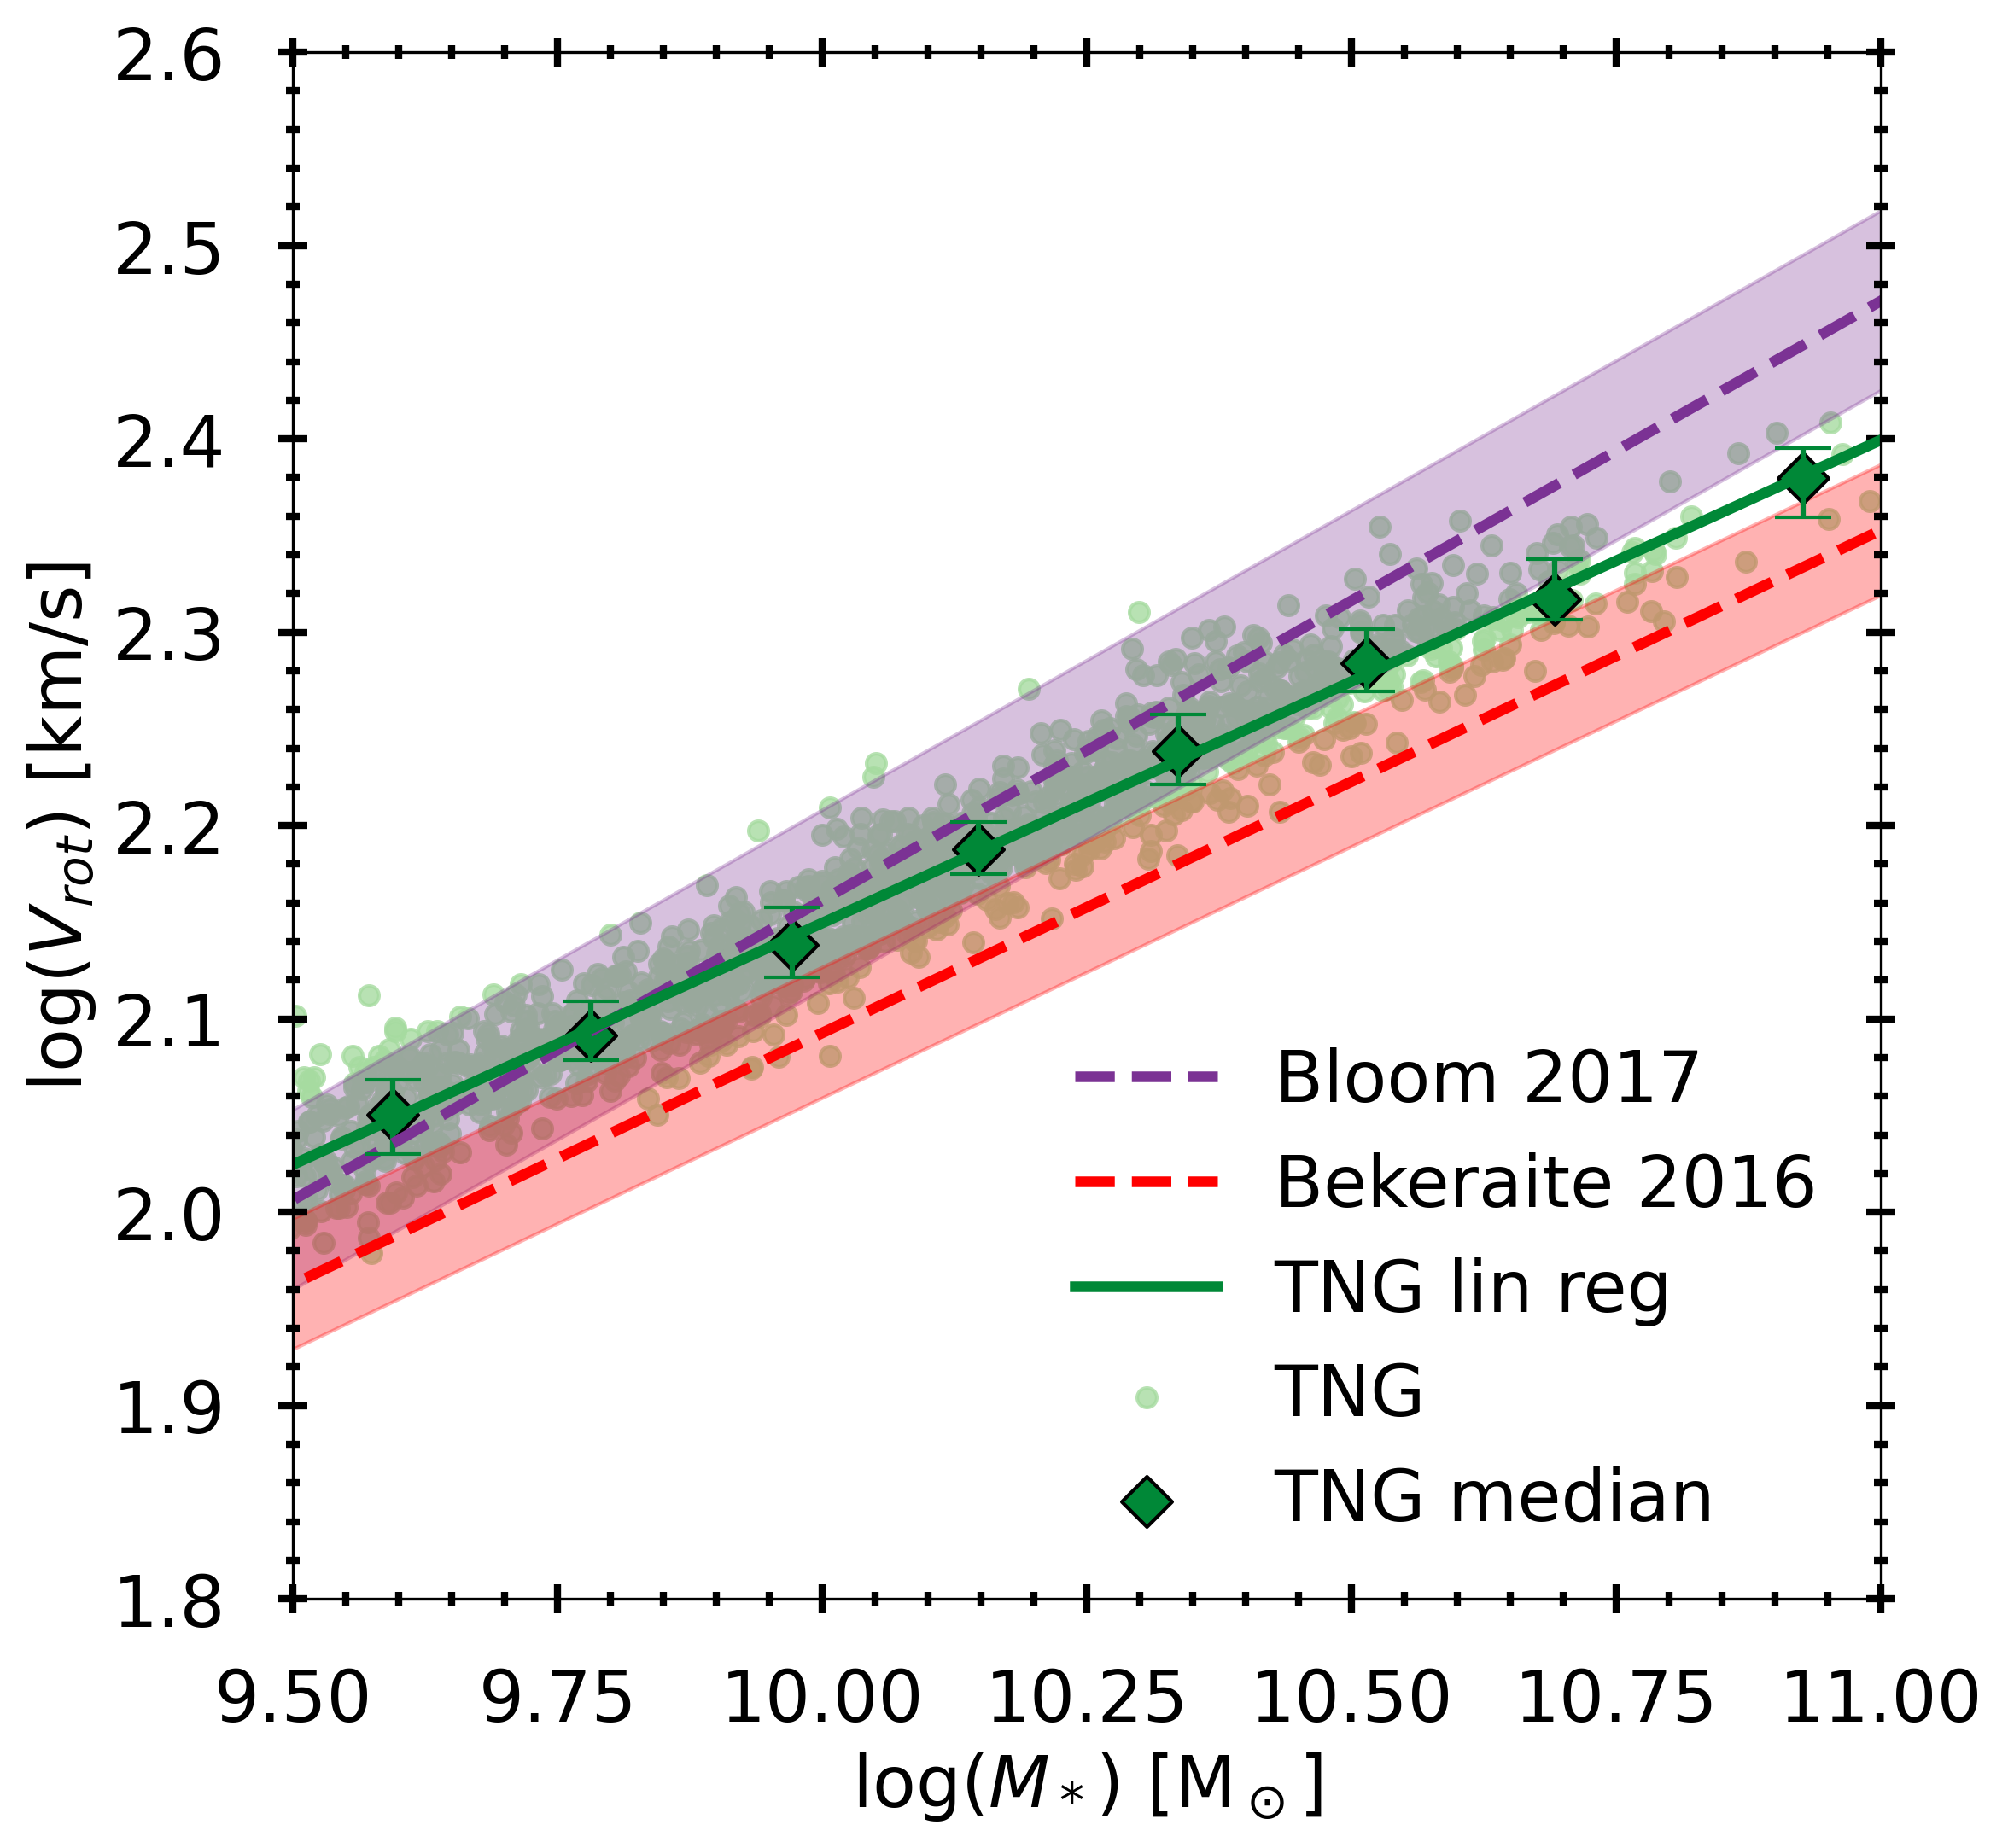
\includegraphics[width=0.9\textwidth]{images/TFR.png}
    \caption{The TFR for TNG (green dots). The median points (green diamonds) for TNG are plotted with error bars, showing the 25-75 percentile. The TNG linear fit is also provided (green solid line). To compare with observations, the best fit for the SAMI data from \textcite{Bloom2017} is shown (purple dashed line) along with the best fit for the CALIFA survey from \textcite{Bekerait2016} (red dashed lline).}
    \label{TFR}
\end{figure}


\subsubsection{Mass - velocity dispersion}
To investigate the difference between using the particles and the SUBFIND catalog for velocity dispersion estimates, several aspects must be considered. The SUBFIND value is the mass averaged velocity dispersion of all particles that are bound to the subhalo ($\sigma^{SUBF}$), and is the only velocity dispersion measurement found in the group catalog. The velocity dispersion measured observationally is either that of stars or that of gas, so using this total velocity dispersion might not give comparable results. In Figure \ref{VD_part} the contribution to $\sigma^{SUBF}$ by stellar, gas and dark matter particles are presented. 
%when you make an analysis of the Figure like this put in brackets which lines/points we have to see in the Figure to follow up those arguments.
%apply to everywhere 
$\sigma^{SUBF}$ is the mass averaged sum of these values, and is higher than the baryonic (gas and stars) velocity dispersions because of the contribution by the dark matter that makes up most of the mass in the subhalo. Gas velocity dispersion is lower than $\sigma^{SUBF}$ by more than 30 \%, and reaching 45 \% in the highest mass galaxies. The stellar velocity dispersion is much closer to $\sigma^{SUBF}$, being approximately equal up to the very largest galaxies where it is less than 10 \% smaller. Looking further at the stellar velocity dispersion in TNG, the effect of a limit on the galaxy size was studied. This is because it might be assumed that velocity dispersion will fall off in the outer parts of the galaxy, and be higher closer to the center. The results show that there is little to no difference in velocity dispersion values for all stellar particles within $0.15 \times r_{200}$ or within 30 kpc compared to the entire subhalo. Observational values are often averaged within $r_e$, so this was also done for TNG, yielding slightly smaller velocities at the high mass end compared to $\sigma^{SUBF}$. The projection effect was also studied by calculating the projected velocity dispersion in three orthogonal directions and comparing it to scaling the 3D velocity dispersion by a factor of $1/\sqrt{3}$. The difference was neglible, as expected for the elliptical early type galaxies.

\begin{figure}
    \centering
    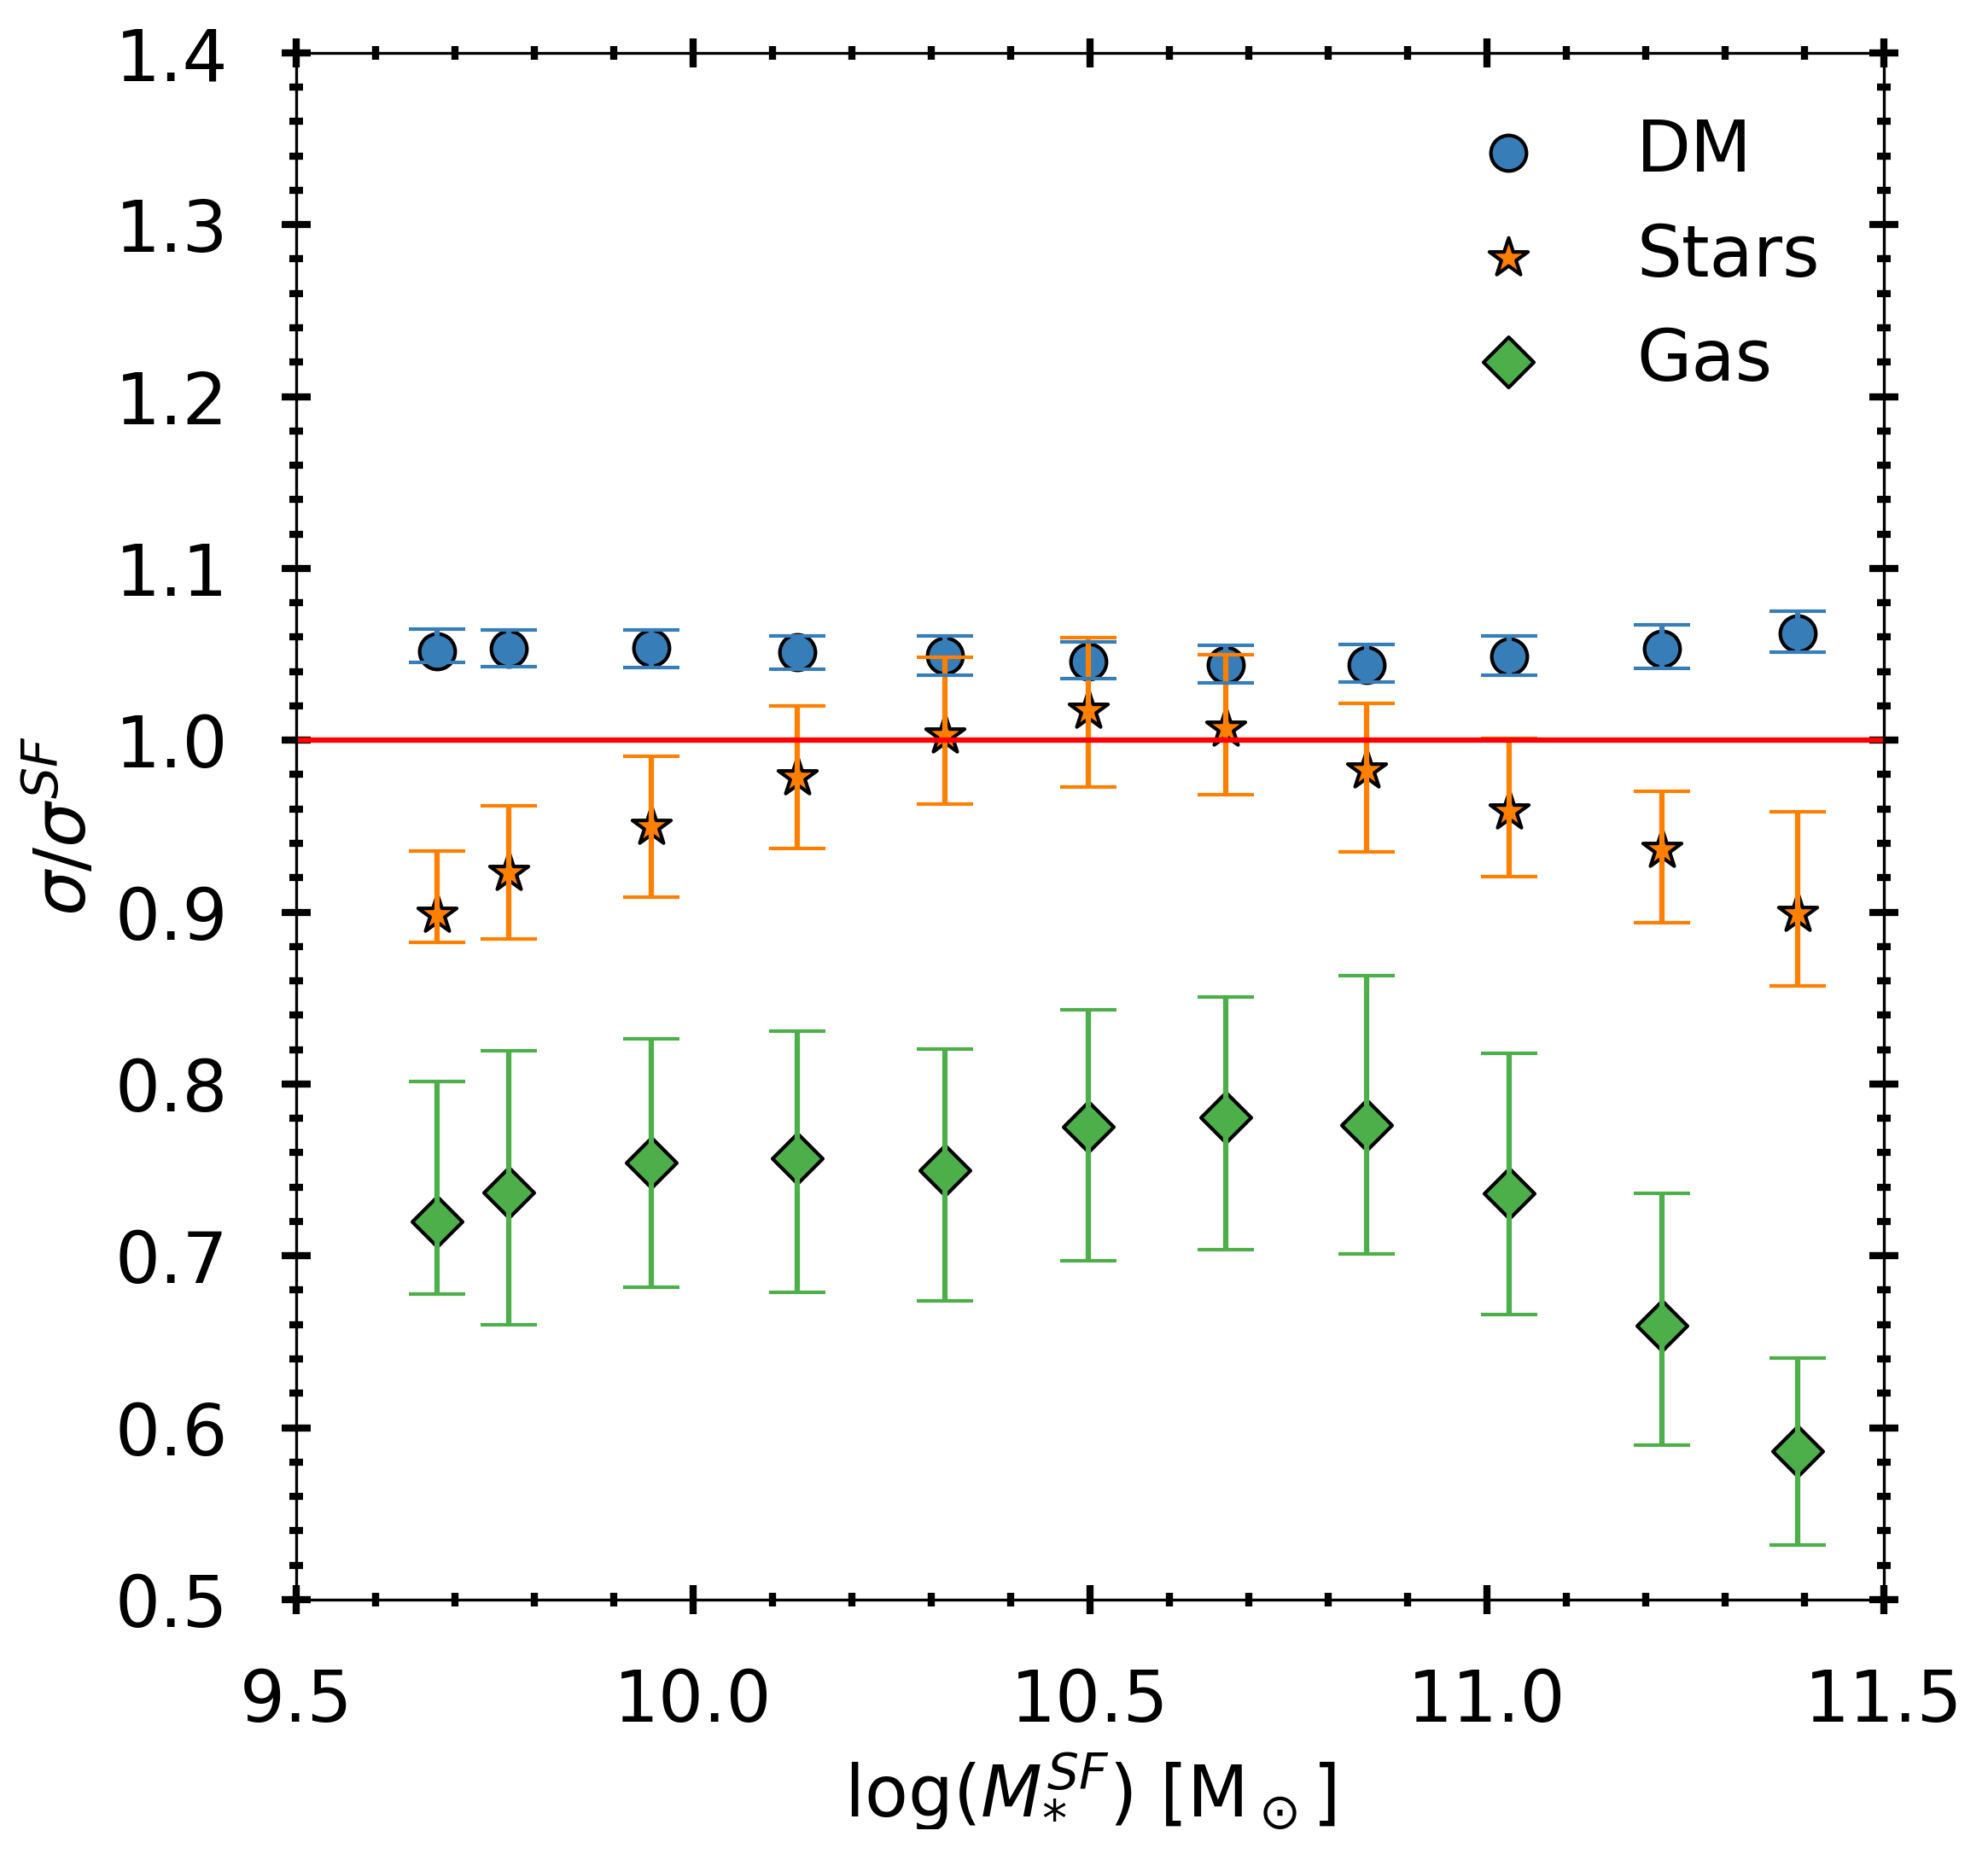
\includegraphics[width=0.9\textwidth]{images/VD_particles.png}
    \caption{Velocity dispersion plotted as function of mass for particles bound to TNG subhalos as identified by SUBFIND. Median values with 25-75 percentile error bars are shown for dark matter (blue circles), stellar particles (orange stars) and gas cells (green diamonds).}
    \label{VD_part}
\end{figure}

The Faber-Jackson relation for early type galaxies is shown in Figure \ref{FJ}. We get lower velocity dispersion in TNG compared to SAMI, by about 0.05 - 0.15 dex. It is tempting to contribute the discrepancy to the difference in stellar mass, however by looking at the SHMR relation in Figure \ref{shmr} we see that the mass deviates from observations at around $10^{11} M_{\odot}$, while in Figure \ref{FJ} the difference starts much earlier. Also, the mass is only off from the observations by about 0.1-0.2 dex, but starting at $10^{10.5} M_{\odot}$ the difference from SAMI in the Faber-Jackson relation is larger, up to 0.4 dex at the highest masses.


\begin{figure}
    \centering
    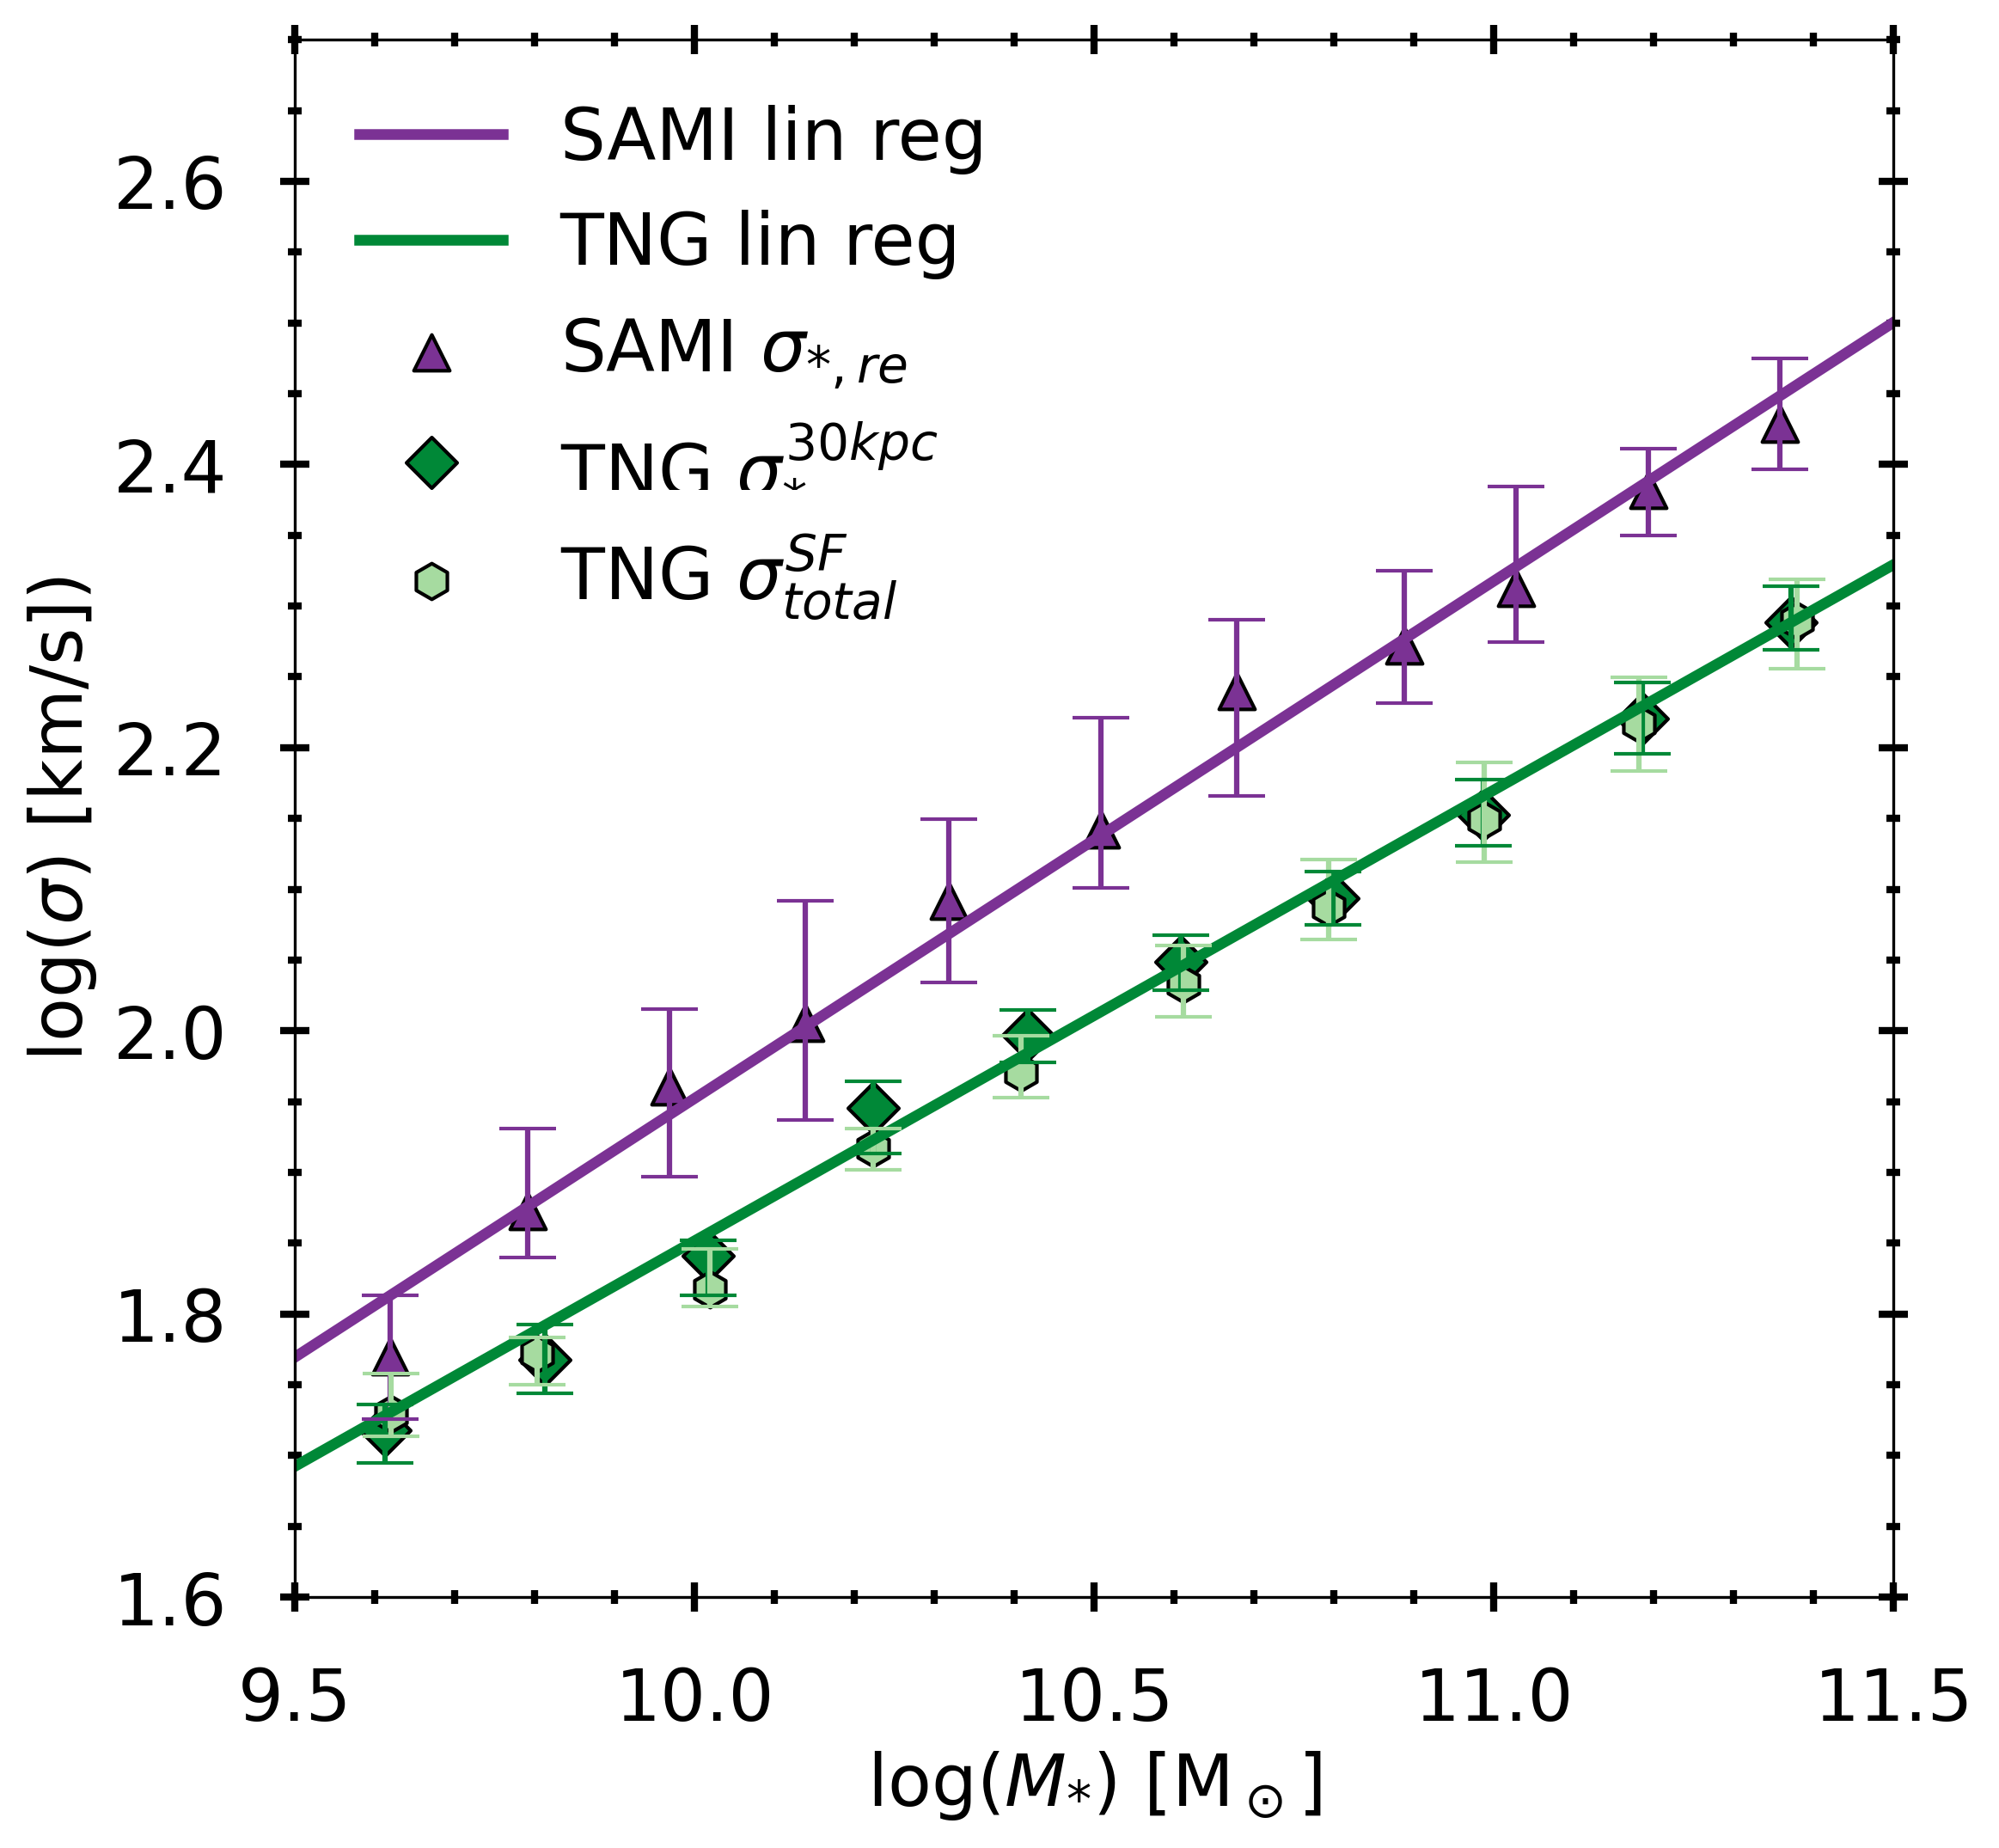
\includegraphics[width=0.9\textwidth]{images/FJ.png}
    \caption{The FJ relation in early type galaxies given by median points with 25-75 percentile error bars for for TNG (dark green points) and SAMI (purple points). Also included are the median points and error bars for the SUBFIND catalog (light green points). The linear fit to TNG (SAMI) are shown as a solid dark green (purple) line.}
    \label{FJ}
\end{figure}



\subsection{Color bimodality}
The final galaxy property which was studied is the color bimodality. Color bimodality is an important feature of observed galaxies, and it has been well documented to be present in TNG galaxies as well \parencite{Nelson2017}. Firstly, the sensitivity to aperture sizes of the g-i color measurements was checked, and there was no apparent difference in the results. This is expected, as the g-i color measures the color of the light that is coming from stars. The larger galaxies, which are the most affected by a limiting aperture, are made up of old stars with very little star formation going on regardless of which part of the galaxy is inspected. The results presented in this Section are therefore those measured within the 30 kpc aperture, as those stellar masses are closer to the observed values in the SHMR. It is also important to mention here that SAMI data contains satellite galaxies as well as centrals, so they will be more affected by environment than TNG galaxies.

The color-mass diagram of the entire galaxy population with $M_\ast > 10^{9.5}M_{\odot}$ for the two data sets is presented in Figure \ref{CB}. The separation into two higher density regions in the blue and red end of the spectrum is obvious for TNG. In SAMI, the separation is less obvious. There is a defined red group, but the blue galaxies are much more spread out compared to TNG. Also, in observations the galaxies tend to get more red as they increase in size, but this slope is much shallower or even flat in TNG galaxies.

In Figure \ref{CB_PDF} the PDF for the g-i colors in early and late type galaxies in TNG and SAMI are shown. The height of the peaks are not comparable, but the distribution and peaks of the color of galaxies are remarkably similar. There is a slight shift towards bluer colors for the peaks in the populations of TNG by about 0.05-0.1 mag compared to SAMI, reflecting the missing upwards trend in the color-mass diagram. 


\begin{figure}
    \centering
    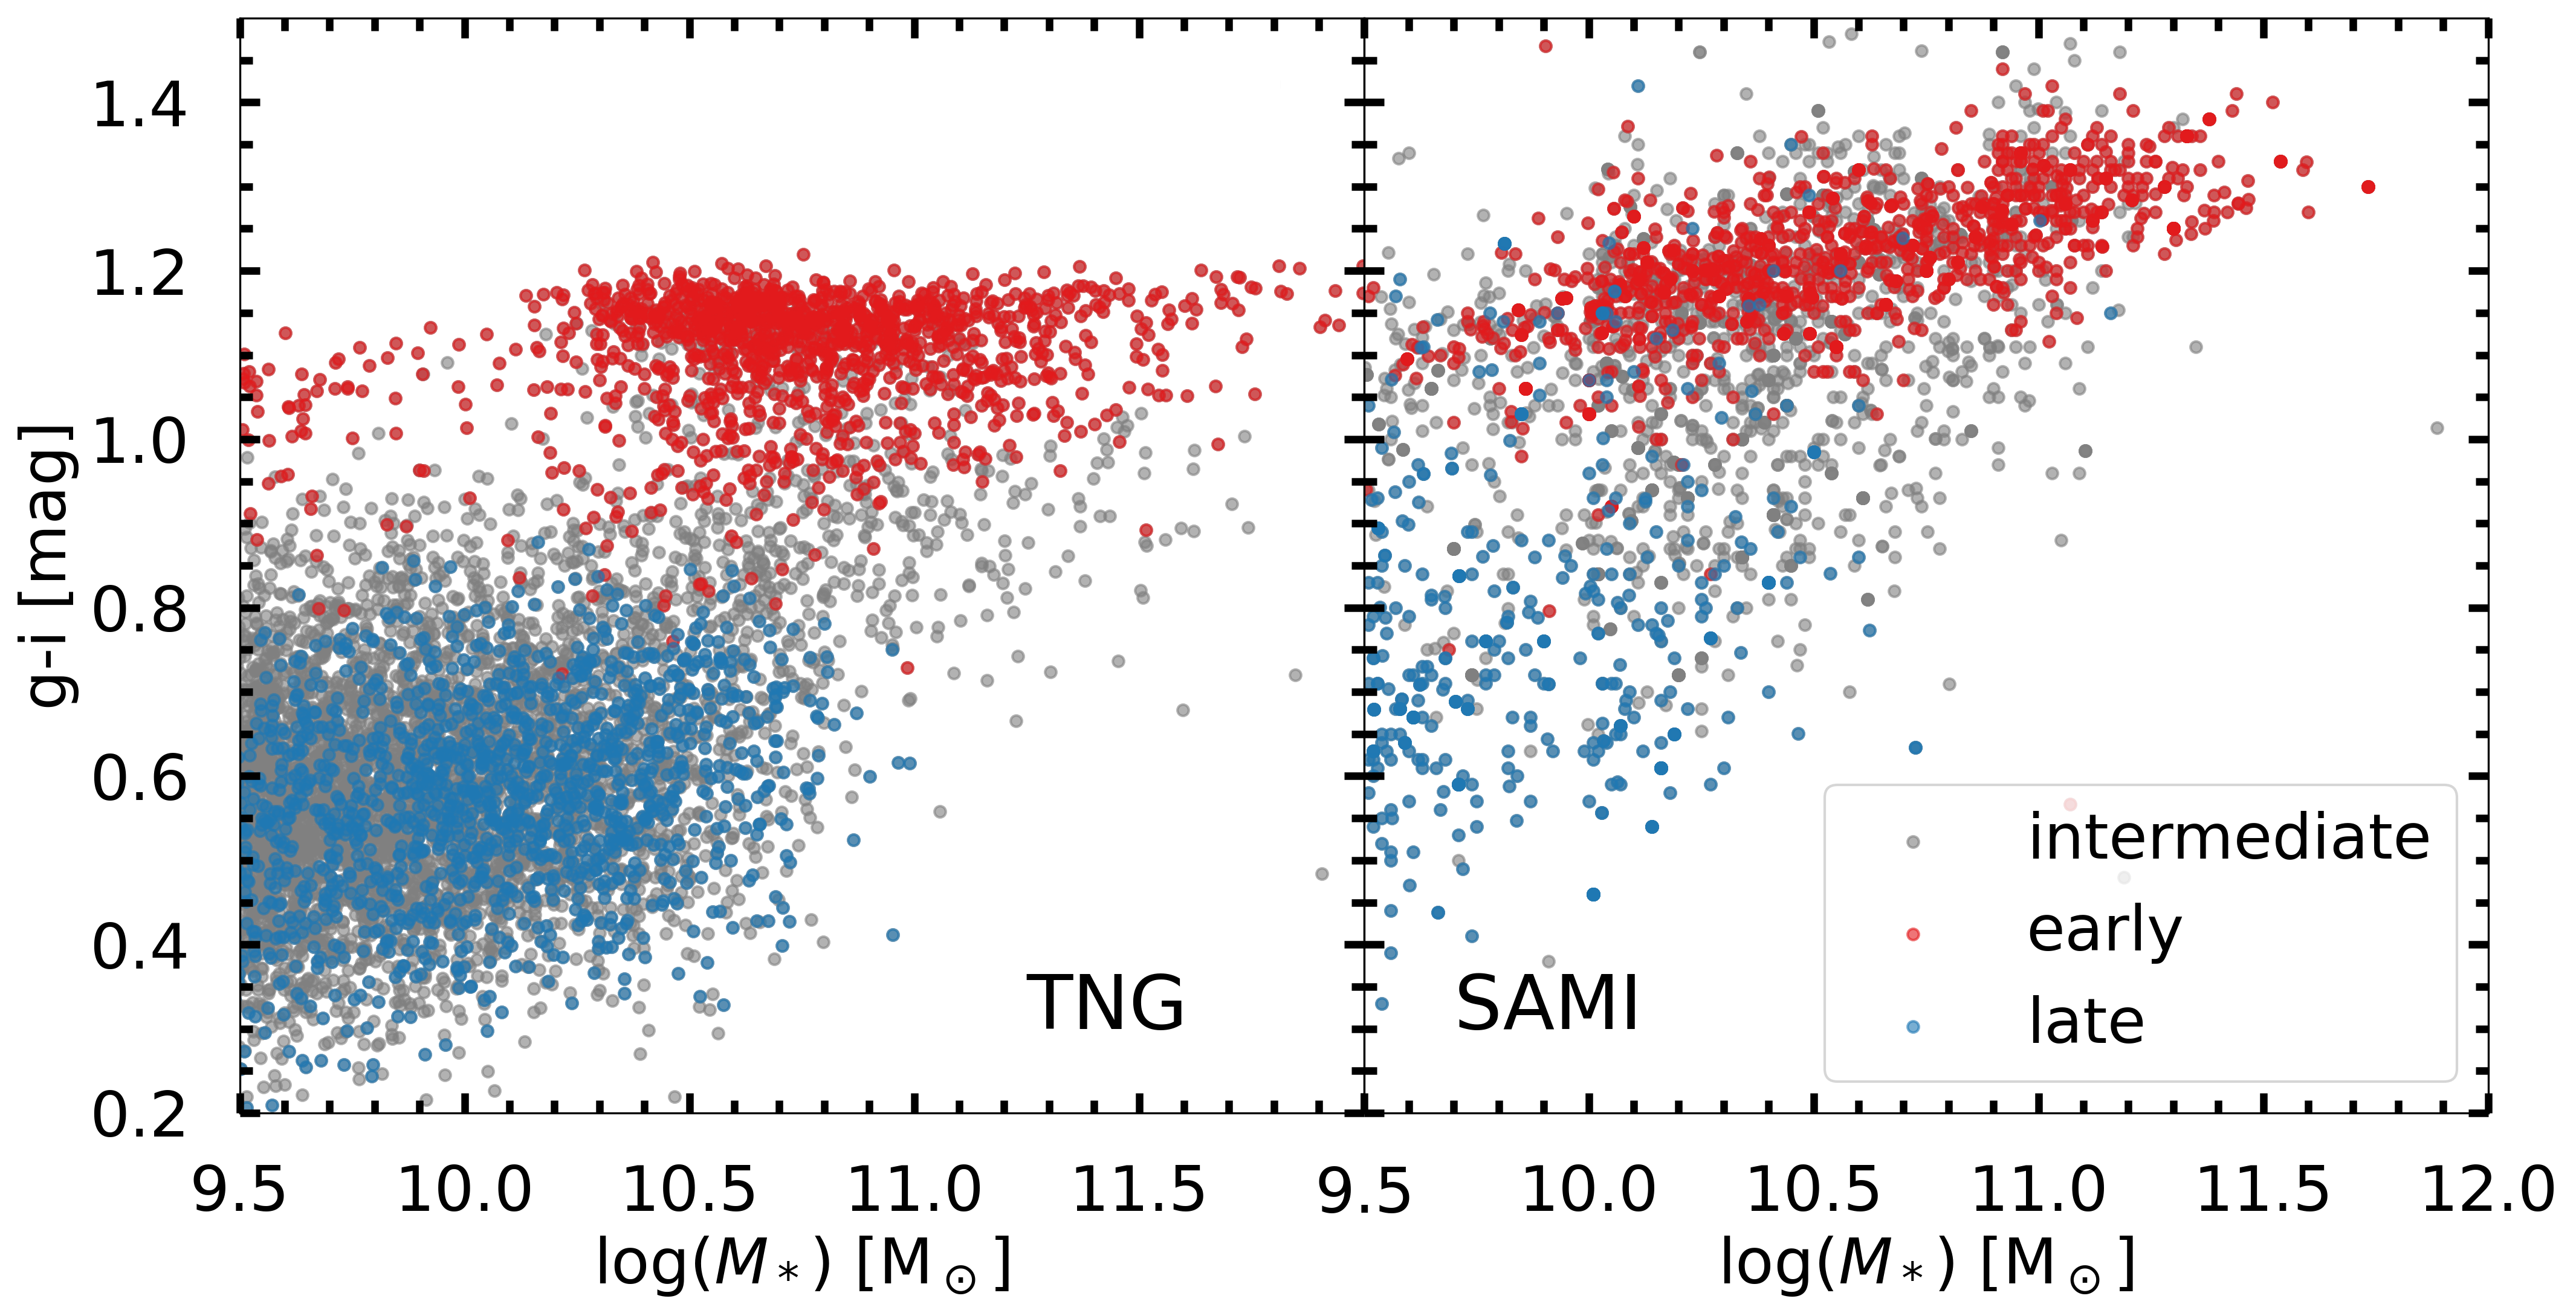
\includegraphics[width=\textwidth]{images/CB.png}
    \caption{Left: Color-mass diagram showing the TNG galaxy distribution for early type (red), late type (blue) and intermediate type (grey) galaxies. Right: Similar color-mass diagram showing the SAMI galaxy distribution.}
    \label{CB}
\end{figure}

\begin{figure}
    \centering
    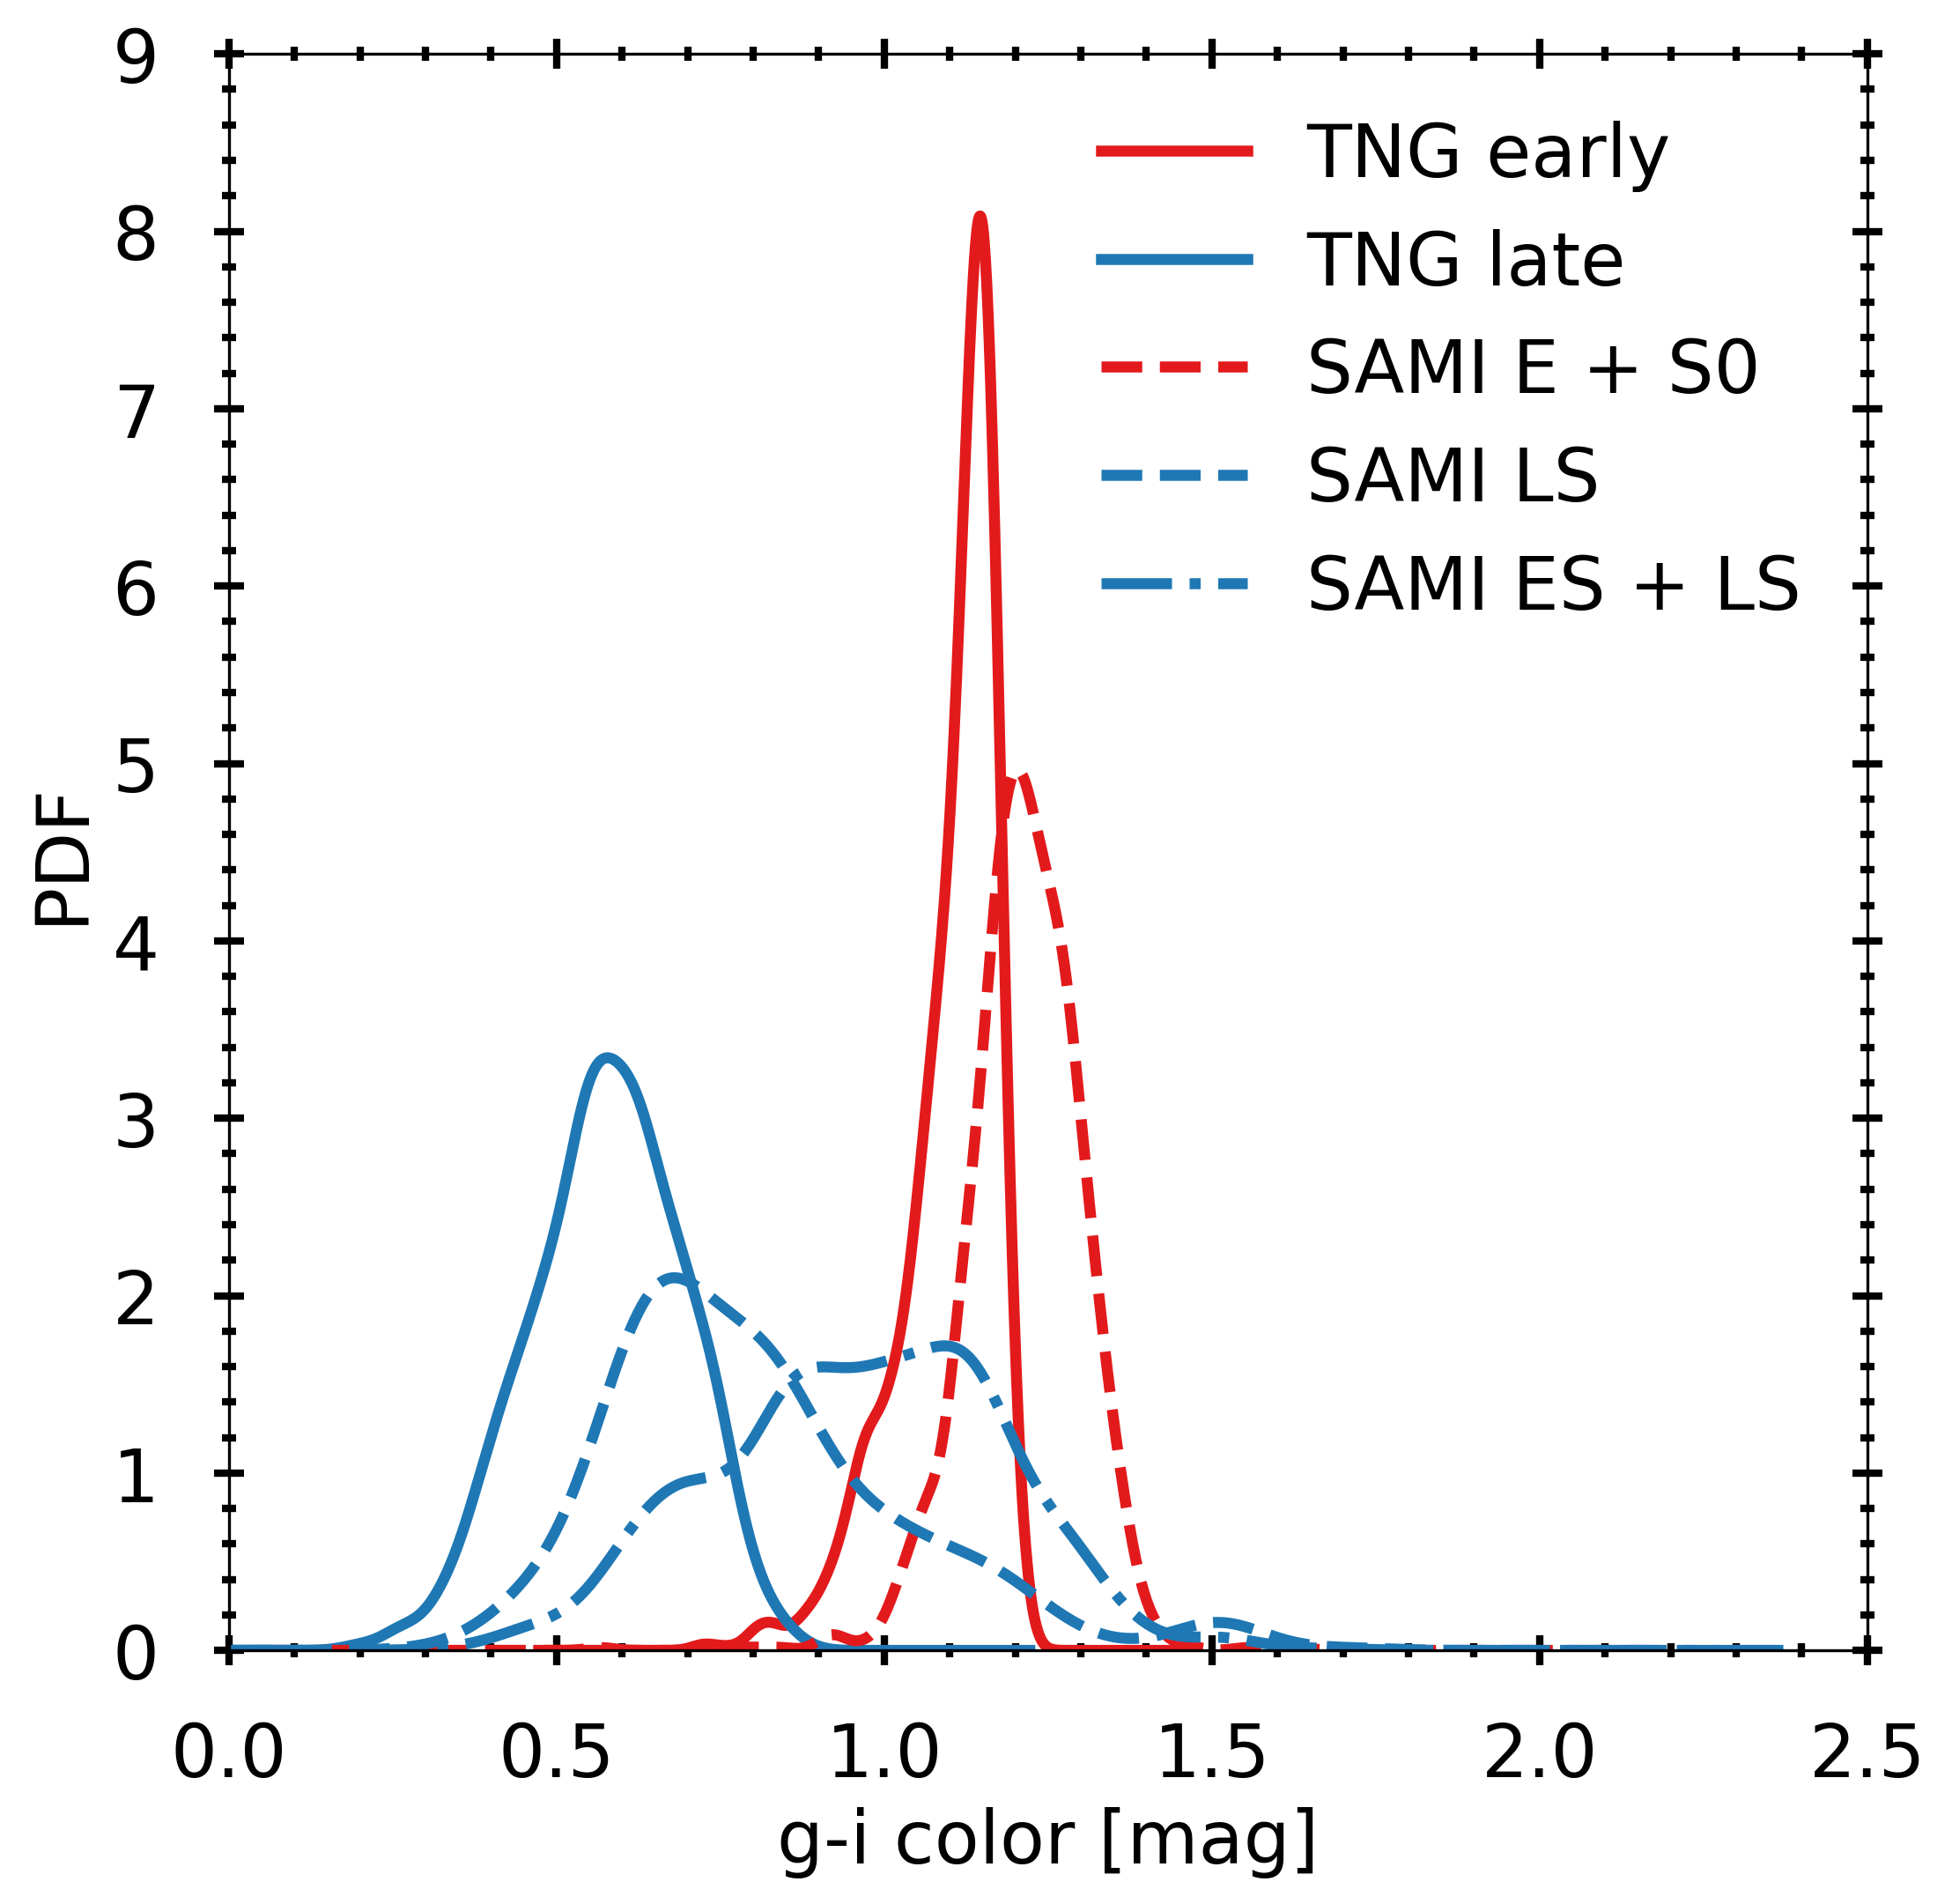
\includegraphics[width=0.9\textwidth]{images/CB_PDF.png}
    \caption{The distribution of g-i color in TNG and SAMI. Kernel density weighted PDF (with Gaussian kernels) are shown for TNG early and late types (red and blue solid lines) as well as for SAMI (red and blue dashed lines). For SAMI late type, two different morphology selections are shown. The short-dashed line show the PDF for the late spiral galaxies and the long-dashed lines show the PDf for the early and late spirals. The values are not normalized, so the height of the peak is not comparable, but the x-position and width is.}
    \label{CB_PDF}
\end{figure}